\documentclass[a4paper, french, 12pt]{article}  % DŽclare la classe du document.
% Il existe 5 classes sous LaTeX : article, book, report, letter et slides 
% Les options de classe sont entre crochets et permettent de faire des choix d'ordre gŽnŽral :
% - dŽfinir la taille de base des caractres avec 10pt, 11pt, 12pt, les commandes d'agrandissement 
% ou de rŽduction de la tailles des caractres ( \small \large ) se feront alors par rapport ˆ cette base
% - dŽfinir la taille du papier:  a4paper,  a5paper, b5paper, executivepaper, legalpaper ou letterpaper
% Utiliser a4paper ds que la papier utilisŽ est de ce format c'est ˆ dire ... tout le temps ;-)
% - utiliser des options de mise en page : 
%       ->   landscape passe en mode paysage pour l'ensemble du doccument
%       ->   onecolumn  option par dŽfaut, le texte sera sur une seule colonne 
%       ->   twocolumn   pour un doccument sur deux colonnes, des rŽglages sont possibles (cf doc & net)
%       ->   oneside toutes les pages seront traitŽs identiquement, par dŽfaut avec la classe article
%       ->   twoside  mise en page diffŽrentes pour les pages pairs et impairs par dŽfaut avec book
%       ->   openright et openany  pour gŽrer le commencement des chapitres dans la classe book
%       ->   titlepage et notitlepage indique si une nouvelle page doit tre commencŽe aprs le titre du document.

% \usepackage permet de dŽclarer un module qui sera pris en compte dans la suite. 
% Les modules permettent d'Žtendre les fonctionnalitŽ de LaTeX

%%%%Caracteres reserves%%%%%%%%%%%
%Pour les obtenir on les fait précéder d'un \
% { s'obtient avec \{
% } s'obtient avec \}
% % s'obtient avec \%
% $ s'obtient avec \$
% & s'obtient avec \&
% # s'obtient avec \#
% _ s'obtient avec \_
% ^ s'obtient avec \^{}
% \ s'obtient avec \textbackslash{} car \\ est une commande
%Les caractères [ et ] ne sont pas réservés et s'obtiennent directement
%\[ et \] delimitent une environnement mathematique
%%%%%%%%%%%%%%%%%%%%%%%%%%%%%%%%%%%%%%%%%%%


%%%%%Polices%%%
%La police employee par defaut par Latex s'appelle Computer Modern

%%%Changement de style de police%%

%Police par defaut {\normalfont ...} c'est une bascule

%Trois familles 
%Romaine par defaut
%sans serif \textsf{..} ou {\sffamily ....}
%typewriter \texttt{..} ou {\ttfamily ....}

%Quatre formes
%droite par defaut
%italique \textit{..} ou {\itshape ....}
%penchee \textsl{..} ou {\slshape ....}
%petites capitales  \textsc{..} ou {\scshape ....}

%Deux series
%normale par defaut
%grasse \textbf{..} ou {\bfseries ....}


%%Taille%%
%Toutes les commandes suivantes sont des bascules a utiliser entre accolades
%{\tiny petit mot}
%Dans l'ordre croissant
%\tiny
%\scriptsize
%\footnotesize
%\small
%\normalsize
%\large
%\Large
%\LARGE
%\huge
%\Huge

%%%%%%%%%%%%%%%%%%%%%%%%%

%%%%%Justification%%%%%
%Alignement a droite
%\begin{flushright}
%{\raggedleft texte \par} ne pas oublier \par
%\leftline{texte}
%\filleft pour formater un titre 

%Alignement a gauche
%\begin{flushleft}
%{\raggedright texte \par} ne pas oublier \par
%\rightline{texte}
%\filright pour formater un titre 


%Centrage
%\begin{center}
%{\centering texte \par} ne pas oublier \par
%\centerline{texte}
%\filcenter pour formater un titre 
%%%%%%%%%%%%%%%%%%%%%%%%%%%%%%%%%%%%%%%%%%%

%%%%%%Espaces%%%%%%%%%%%%%%%%%%%%%


%%Espaces verticaux%%%
%\vskip 2cm  (argument eventuellement negatif), l'espace est ignore s'il coincide avec un saut de page
%\vspace*{2cm} (argument eventuellement negatif), l'espace n'est pas ignore s'il coincide avec un saut de page
%\vspace{2cm} est synonyme de \vskip 2cm 

%%Espaces horizontaux%%%%

%\hskip equivalent a \vskip
%\hspace{?} et \hspace*{?}
%Le cadratin est un espace horizontal egal a la taille de la police utilisee
%\thinspace espace d'un sixieme de cadratin
%\enskip pour un demi-cadratin
%\quad pour un cdratin
%\qquad pour deux cadratins

%%%%%%%%%%%%%%%%%%%%%%%%%%%%%%%%%%%%

%Le moteur eTeX est aujourd'hui utilisé par toutes les distributions (MikTeX, TeXlive) à la place de l'ancien TeX (en fait, c'est plutôt PDFTeX, le successeur de eTeX, qui est utilisé ; contrairement à ce que son nom indique, il peut produire du dvi). Le fait d'utiliser le moteur eTeX au lieu de TeX donne accès à des choses en plus (par exemple à \middle pour aller avec \left et \right, mais aussi à des commandes bien pratiques comme \numexpr, \dimexpr, \detokenize, etc. ainsi qu'à des ressources supplémentaires, comme plus de compteurs disponibles).

%Lorsqu'on utilise le moteur eTeX, certaines de ces fonctionnalités sont automatiquement accessibles (c'est le cas de \middle, \numexpr, etc.), mais pas d'autres (c'est le cas des compteurs supplémentaires). Pour activer ces fonctionnalités manquantes, on peut charger le package etex.sty. Ainsi, l'utilisation d'etex.sty est une solution courante au problème d'avoir trop de compteurs définis (c'est le cas si on charge ensemble trop de packages du type tikz, pstricks, xymatrix, ...)

\usepackage{etex}

%%%%%%%%%%%%Encodage du fichier source %%%%%%%%%%%
\usepackage[T1]{fontenc}
\usepackage[utf8]{inputenc}


%%%%%%%%%%%%%%%Francisation%%%%%%%%%%%%%%
\usepackage[french]{babel}
\frenchbsetup{StandardLists=true}
%%%%%%%%%%%%%%%%%%%%%%%%%%%%%%%%%%%%%%%%%

%%%%%%%%%%%%Mise en page, Reglages genrraux%%%%%%%

%\title{il n'existe pas de plus grand nombre premier}
%\author[Euclide \thanks{Merci Aristote}}
%\date{12 juin $-260$}  Par défaut Latex insère la date du jour
%puis écrire après \begin{document} la commande \maketitle


\usepackage[a4paper,headheight=35 pt, headsep=15pt,top=20 pt,hmargin=1 cm,bottom=20 pt,includeheadfoot]{geometry}
%\usepackage[a4paper,hmargin=1 cm,bottom=2cm,top=2cm,headheight=15pt]{geometry}      
%top est la marge supérieure entre le haut de body et le bord supérieur de la feuille
% \usepackage[left= 4cm,right = 3cm,top= 2cm, bottom=2cm]{geometry} pour le réglage des marges 
% \usepackage[top= 17mm,textheight=23cm,heightrounded,left=25mm,textwidth=16cm] {geometry} pour fixer la hauteur,  la largeur  du texte. heightrounded, autorise le package à arrondir la hauteur textheight à un nombre entier de lignes pour éviter des problèmes de remplissage vertical underfull vbox 


\usepackage{setspace}  % pour le réglage de l'interligne
%Bascule \doublespacing  ou environnement {doublespace}
%Bascule \onehalfspacing  ou environnement {onehalfspace}
%Bascule \singlespacing  ou environnement {singlespace}
% ou encore \renewcommand{\baselinestretch}{n} ou encore l'environnement spacing{n}

%%Package fullpage
%\usepackage[cm]{fullpage}
%where possible options for fullpage are
%in (default) sets the margins to one inch;
%cm sets the margins to 1.5 cm (one centimeter is really too
%little);
%plain (default) selects the plain page style, i.e., with no head-
%ers but only a footer;
%empty for neither headers nor footers;
%headings for both header and footers;
%myheadings also for both headers and footers.
%For the last 4 options, the corresponding \pagestyle declaration is exe-
%cuted, so that it is not necessary to give it again.


%%Pour la numerotation des bas de pages avec le compteur lastpage%%%
\usepackage{lastpage}

%%%%Pour afficher certaines pages au format paysage%%
\usepackage{lscape}
%\begin{landscape}

%%%Plusieurs colonnes
\usepackage{multicol}
%\begin{multicols}[titre]{nb colonnes}
\setlength{\columnseprule}{0.25pt}


%%%%%Références, Notes de bas de pages ou de marges%%%%%%%%%

%%Pour placer une note de bas de page : commande \footnote{}
%Pour placer une note dans la marge : \marginpar{}
%Pour plcaer une note dans un tableau : appel de note avec \footnotemark{} puis le texte après le tableau avec \footnotetext{texte}

%Etiquette  avec \label{nom} puis référence à l'étiquette (numéro de section le plus proche ) avec \ref{nom} ou à lap age avec \pageref{nom}
\usepackage{varioref}
%Introduit  les commandes \vref{} et \vpageref{} qui améloirent l'affichage ainsi que la commande \vpagerefrange{label1}{label2} pour faire référence à tout un bloc de pages entre deux étiquettes
\usepackage{nameref}


%%%%Présentation des titres de section%%%

%\usepackage[clearempty]{titlesec} problème avec PDFLatex ?

%Pour changer la police des titres de sectionnement, un exemple :
%\titleformat*{\section}{\sffamily}

%Pour modifier la police mais aussi la présentation :
%\titleformat{commande}[shape]{format}{label}{sep}{before}{after}
% commande est la commande de sectionnement comme \section
%shape peut etre hang (défaut),frame (encadre), display( paragraphe séparé), block (paragraphe), runin (dans le texte, wrap (comme wrapfigure), leftmargin ou rightmargin
%format est le formatage du titre complet (numéros inclus)éventuellemnt précédé de commandes à inclure avant le titre
% Ces commandes peuvent etre \titleline[r,c ou l]{texte} ou \titlerule[epaisseur] ou \titlerule*[epaisseur]{texte}
%label est la présentation du numero
%sep est l'espace entre le numero et le titre
%before est le code à exécuter avant le titre de section (numero exclu)
%after est le code à exécuter après (vide en général)

%Pour gérer l'espacement
%\titlespacing{commande}{left}{beforesep}{aftersep}[right]
%left est la marge à gauche, beforesep l'espace vertical avant etc ..


%Exemple de présentation de titre encadé :
%\titleformat{\section}[frame]{\titleline[r]{\rule{2in }{2pt}} \normalfont}{\filright\small\ SECTION \thesection\hfill}{7pt}{\LARGE \bfseries\filcenter}{}
%\section{un titre de section encadre}


%%%%%%%%%%%%%%%%%%%%%%%%%%%%%%%%%%%%%%%%%%%% 

%%%%%%%Réglages de la table des matières%%%%
\usepackage{tocvsec2}
%Définir la progondeur : \setcounter{tocdepth}{1}  :
%1 correspond aux chapitres; 2 aux sections etc ...
%Rédéfinir le nom par défaut  :
%\renewcommand{\contentsname}{Liste des chapitres}
%Modifier une entrée :
%\Chapter[titre court]{titre long}
%Ajouter une entrée :
%\addcontentsline{toc}{section}{Nom de la section qu'on veut ajouter}
%Pour exclure une entrée 
%Utiliser une commande étoilée comme \section*
%Pour ajouter  ce qu'on veut dans la table des matières comme des indications de mise n page :
%\addtocontents{toc}{\protect \pagebreak}


%%%%%%%%%%%% Packages pour le texte %%%%%%%%%%%%
\usepackage{lmodern}       %Joli fonte

\usepackage{pifont,fourier}
\usepackage[normalem]{ulem}
%\uline{} pour  un soulignement simple
%Commmandes \uuline{} pour un soulignement double
%\uwave{} pour un soulignement  avec des vagues
% \sout{} pour barrer et \xout{} pour hachurer
\usepackage[thicklines]{cancel} %Commande \cancel{} pour barrer en oblique
\usepackage{soul}    %souligner avec \ul
%\usepackage{lettrine} %Pour commencer un paragraphe avec une lettrine
%Package incompatible avec tabvar.tex
%\lettrine{S}{i vous souhaitez}
%\renewcommand{\LettrineFontHook}{\itshape}
%\renewcommand{\LettrineTextFont}{\sffamily}

%%%Pour des jolis boites%%%
\usepackage{fancybox}  
%Commandes \box{} \ovalbox{} \shadowbox{}
%\cornersize{}2 réglage de l'arrondi
% Dimension à régler avec \setlength{}  : \fboxsep \fboxrule  

%%% Pour faire tourner le texte %%%
\usepackage{rotating}  %\begin{turn}{-60} tourné \end{turn} pour tourner un paragraphe
						%pour tourner un texte, commande \rotatebox[origin=c]{angle}{texte}
						
%%Divers%%%%
\usepackage{eurosym}  %pour le symbole de l'euro

\usepackage{url} %pour la gestion des adresses web avec la commande \url{}

%%%%%%%%%%%

%%%%%%%%%%%%%%%Ecriture d'algorithmes Insertion de code source %%%%%%%%%%%

%%%%%Package verbatim%%%%

\usepackage{verbatim} 
%LE package verbatim améliore la présentation des verbatim
% Il  fournit un environnement {comment} pour insérerer des commentaires
%dans le fichier source sans faire précéder toutes les lignes de %

\usepackage{alltt, moreverb} 
%L'environnement verbatimboxed permet d'encadrer un texte en verbatim
% De plus les caractères spéciaux \ et { ne sont pas désactivés (mais #, $ et % le sont)
% et on peut saisir des formules mathématiques avec \( .. \) ou \[ ... \]

%%Pour améliorer envore la présentation des verbatim%%%%
\usepackage{fancyvrb}


%%Couleur
\usepackage[table,svgnames]{xcolor}
% options : rgb,cmyk,gray,hsb,html pour transformer automatiquement toutes les couleurs du docuement dans le mode choisi
%\definecolor{mauve}{rgb}{0.7,0,0.43}
%\color{couleur} bascule
%\textcolor{couleur}{texte}
%\pagecolor{couleur}
%\colorbox{couleur}
%\fcolorbox{couleur}




%%%%%%%%%% Nouvelles couleurs
\definecolor{rouge}{rgb}{1,0,0}
\definecolor{bleu}{rgb}{0,0,1}
\definecolor{orange}{rgb}{1.00,0.50,0.00}
\definecolor{vert}{rgb}{0,0.50,0.00}
\definecolor{marron}{rgb}{0.49,0.16,0.06}
\definecolor{mauve}{rgb}{0.42,0.24,0.77}
\definecolor{rpastel}{rgb}{1.00,0.77,0.77}
\definecolor{bpastel}{rgb}{0.70,0.86,0.93}
\definecolor{grisclair}{gray}{0.85}
\definecolor{gristclair}{gray}{0.95}
\definecolor{grisfonce}{gray}{0.4}

%%%%%%%%%%%%%%%%%%¨Puce, Listess%%%%%%%%%%%%%%
\usepackage{enumerate}
\usepackage{enumitem}
%Pour changer la puce de liste dans tout le document :
%AtBeginDocument{\renewcommand{\labelitemi}{\textbullet}}
%%%%%%%%Réglages spécifiques au document%%%%%%%%%

%\setenumerate[1]{label=\textbf{Q\arabic*)}}

%Listes en colonnes / QCM
\usepackage{tasks}
\DeclareInstance{tasks}{multiplechoice-box}{default}{
label= $\Box$,
label-width=15pt
}
\DeclareInstance{tasks}{multiplechoice-alph}{default}{
label=\underline{Réponse \Alph* :},
label-width=65pt,
label-format=\bfseries
}

\settasks{
item-indent = 60pt
}
%%%%%%%%%%%%Graphiques et Dessins%%%%%%%%%%%%%%

\usepackage{graphicx}		
%\rotatebox[origin=x0x1]{angle}{texte} avec xox1 parmi t (top) l (left) r (right) B (ligne de base) et b (bottomm)
%\resizebox{largeur}{hauteur}{texte} pour faire rentrer u nelement encombrant dans une boite					


\usepackage{epic,eepic}   %Capacités graphiques étendues
%\begin{picture}(0,0) permet d'insérer n'importe quoi, n'importe où sans prendre de place (utilie pour annoter une figure en eps)
%Une autre technique est \makebox[0cm][alignement]{texte}
%Exemple:
%\includegraphics[scale=1]{singe.eps}
%\begin{picture}(0,0)
%\put(-27,10){$\sqrt[3]{8}$}
%\end{picture}



%%%%%%%%%%PSTricks%%%%%%%%%%%%

\usepackage{pstricks,pst-plot,pst-text,pst-tree,pst-eps,pst-fill,pst-node,pst-math,pstricks-add,pst-xkey,pst-eucl}


%%%%%%%Tikz%%%%%%%%%%%%%%%
\usepackage{pgf,tikz,tkz-tab}
% Pour les tableaux de signes ou de variations avec tkz-tab voir https://zestedesavoir.com/tutoriels/439/des-tableaux-de-variations-et-de-signes-avec-latex/#1-13389_tikz-un-package-qui-en-a-dans-le-ventre
\usetikzlibrary{arrows}
\usetikzlibrary{shapes.geometric}
\usetikzlibrary{shapes.geometric}
\usetikzlibrary{petri}
\usetikzlibrary{decorations}
\usetikzlibrary{arrows}
\usetikzlibrary{math}
 %Variables must be declared in a tikzmath environment but
       % can be used outside
%       \tikzmath{int \n; \n = 508; \x1 = 1; \y1 =1; 
%                   %computations are also possible
%                    \x2 = \x1 + 1; \y2 =\y1 +3; } 


%%%%%%%%%%%%%%%%%%%%%%%%%%%%%%%%%%%%%%%%
%%%%%%%%%%%Commandes Tikz Perso%%%%%%%%%%%%%%%

% Définition des nouvelles options xmin, xmax, ymin, ymax
% Valeurs par défaut : -3, 3, -3, 3
\tikzset{
xmin/.store in=\xmin, xmin/.default=-3, xmin=-3,
xmax/.store in=\xmax, xmax/.default=3, xmax=3,
ymin/.store in=\ymin, ymin/.default=-3, ymin=-3,
ymax/.store in=\ymax, ymax/.default=3, ymax=3,
}
% Commande qui trace la grille entre (xmin,ymin) et (xmax,ymax)
\newcommand {\grille}[2]
{\draw[help lines,black, thick] (\xmin,\ymin) grid[xstep=#1, ystep=#2] (\xmax,\ymax);}
% Commande \axes
\newcommand {\axes} {
\draw[->,very thick] (\xmin,0) -- (\xmax,0);
\draw[->,very thick] (0,\ymin) -- (0,\ymax);
\draw (0.95*\xmax, 0) node[above] {$x$};
\draw (0, 0.95*\ymax) node[left] {$y$};
}
% Commande qui limite l?affichage à (xmin,ymin) et (xmax,ymax)
\newcommand {\fenetre}
{\clip (\xmin,\ymin) rectangle (\xmax,\ymax);}

%Exemple d'utilisation

%\begin{center}
%\begin{tikzpicture} [xmin=-2,xmax=2,ymin=0,ymax=5]
%\grille{1} \axes \fenetre
%\draw plot[smooth] (\x,\x^2);
%\end{tikzpicture}
%\end{center}

%style pour la perspective cavalière française
%voir Tikz pour l'impatient page 68
\tikzset{math3d/.style=
{x= {(-0.353cm,-0.353cm)}, z={(0cm,1cm)},y={(1cm,0cm)}}}

%%%%%%%Symbole pour code calculatrice%%%%%%

%Flèche remplie pour défilement de menu

\newcommand{\flechefillright}{
\begin{tikzpicture}[scale=0.15] \fill (0,0)--(2,1)--(0,2)--cycle;
\end{tikzpicture}}

%%%%%%%%%%%%%Symboles pour calculatrice Casio%%%%
\newcommand{\execasio}{\Pisymbol{psy}{191}} %Retour chariot
\newcommand{\dispcasio}{\begin{pspicture}(.1,.1)\pspolygon*(.1,0)(.1,.1)\end{pspicture}} %Triangle « Disp »
\newcommand{\dispcasiotikz}{\begin{tikzpicture}[scale=0.2]
\fill (0,0) -- (1,0) -- (1,1) -- cycle;
\end{tikzpicture}} %Triangle « Disp »
%

%Fleche entre deux lignes, d'apres 'un bon petit' : http://forum.mathematex.net/latex-f6/fleches-entre-deux-lignes-pour-resolution-d-equation-t10283.html#p99817
\newcommand\addnode[1]{\Rnode{#1}{}}
\newcommand\linknode[3]{\ncbar[angleA=0,angleB=0,nodesep=1ex,arm=10ex,offset=-2pt]{->}{#1}{#2}\Aput{\vphantom{x}#3}}


%%Commande pour touche de calculatrice

\newcommand\tc[1]{%
{
\begin{tikzpicture}
\node[draw,rectangle,rounded corners=3pt] (P) at (0,0){#1};
\end{tikzpicture}
}
}

%%%%%%%%%%%%%%%%%%%%%%%%%%%%%%%%%%%%%%%%
%%%%%%%%%%%Fin Commandes Tikz%%%%%%%%%%%%%%%


%%%%%%%%%%%%Specifiques%%%%%%%%%%%
\usepackage{wrapfig}
%pour insérer une figure à droite ou à gauche d'un texte
%\begin{wrapfigure}[nb lignes]{placement l,r,c,i(inside),o(outside)}[overhang]{width}
%ce package fonctionne mal à proximité des listes
%%%%%%%%%%%%%%%%%%%%%%%%%%%%%%%%%%%%%

%%%%%Environnements et symboles spéciaux pour faire joli%%%%%%

%%%Bclogo, pour des environnements + jolis avec insertion de logo%%%%
%Dépendances de  bclogo
\usepackage{xkeyval}  
\usepackage{etoolbox}
\usepackage{ifpdf}
\usepackage[framemethod=tikz]{mdframed}
\usepackage[tikz]{bclogo}

%\newcommand\bcpython{
\includegraphics[width=17pt]{/home/fjunier/Maths/python-logo.eps}}
\newcommand\bcpython{
\includegraphics[width=17pt]{/home/fjunier/Maths/python-logo.png}}
%\newcommand\bcpython{
\includegraphics[width=17pt]{/home/frederic/Maths/python-logo.png}}

%% Framed
\usepackage{framed}  %Le package « framed» Crée 3 nouveaux environnements, qui se comportent comme des minipage de largeur \linewidth, mais permettant en plus de se casser entre plusieurs pages.     * framed : avec un cadre autour;     * shaded : avec un fonc coloré (il faut définir la couleur shadecolor);     * leftbar : avec une barre le long du côté gauche.

%%%%%%%%%%%%%%%%%%%%%%%%%%%%%%%%%%%


%%%%%%Environnements et symboles mathématiques%%%%

%%%%%%%%%% Package ProfCollege %%%%%
%\usepackage{ProfCollege}


%%%Tableaux de variations %%%%%%%%%%

\usepackage{variations}

%%%%%%%%%%%AmsMaths%%%%%%
\usepackage{mathtools}        %Commandes essentielles, extension d'amsmath
\usepackage{amsfonts,amssymb}  %Principaux symboles
\usepackage{mathrsfs} %Polices calligraphiques
\usepackage{stmaryrd} %Pour les intervalles d'entiers avec \llbracket et \rrbracket
\usepackage[autolanguage, np]{numprint}
%%%%%%%%%%%%Là encore il y a de grosses différences entre le monde anglo-saxon et les francophones.Le séparateur des décimales est un point en anglais et une virgule en français. Leséparateur des milliers est une virgule en anglais et une espace insécable en français. Ilest préférable d’utiliser le package numprint (\usepackage{numprint}) qui associé àfrenchb produira la bonne typographie.
%123456789 = 123456789 \numprint{123456789} = 123 456 789  \numprint{3,1415926535897932384626} = 3,141 592 653 589 793 238 462 6  \numprint{12.34} = 12,34  En plus tu peux préciser les unités de cette façon : \numprint[kg]{12.34} = 12,34 kg ou encore \numprint[\degres C]{22} = 22°C Si tu veux utiliser le raccourci \np{} au lieu de \numprint{}, il te faut charger le package de cette façon : \usepackage[np]{numprint}
\usepackage[thmmarks,amsmath]{ntheorem}
%Pour définir un nouveau théorème :
%\newtheorem{conj}{Conjecture}[chapter] environnement con d'en tete Conjecture avec numérotation au sein d'un chapitre
%Pour rédéfinir le style d'un théorème, placer les commandes avant \newtheorem et entourer le tout d'accolades
%\theoremstyle{style} : :
% plain est le style par défaut
% break insère un saut de ligne après le titre du théorème
%margin et marginbreak sont les équivalents avec numéro dans la marge
%\theorembodyfont{\normalfont \sffamily} police du corps du théorème
%\theoremheaderfont{\scshape} police de l'en-tete (définie 1 fois pour tous les théorèmes)
%\theoremsymbol{ } symbole ajouté à la fin du théorème
%\theoremseparator{--} élément situé entre le numéro et le corps du theoreme
%\theoremprework{\rule{\linewidth}{0.4pt}} élément précédant chaque théoreme
%\theorempostwork{\dingline{71}} élément suivant chaque théoreme
%\theoremnumbering{Roman} style de numérotation
\usepackage{bbm, dsfont}   %Fonction indicatrice
\usepackage{esint,esvect}  %Flèches supplémentaires.
\usepackage{lcg}  %%%%%%%générer des nombres pseudo aléatoires%%%%


%%%%%%%%%%%Tableaux%%%%%%%%%%%
\usepackage{array}
%\usepackage{multirow} %problème redéfinit la commande \multirow{nligne}*{texte}
\usepackage{tabularx}        % Largeur totale donnée          
\usepackage{longtable}       %Sur plusieurs pages
%\usepackage{diagbox}  %Successeur de slashbox, voir Latex pour l'impatient p. 73, charge pict2e qui redefinit \arc
\usepackage{alterqcm} 
%%%Une commande de David Robert%%%%%%%
%\newcommand{\delair}[1]{\ensuremath\displaystyle\psframebox[framesep=0.15em,linestyle=none]{ \displaystyle#1}}
\newcommand{\delair}[1]{\setlength{\fboxrule}{0mm} \fbox{#1}}
%%%%%%%%%%%%%%%%%%%%%%%%%%%%%%%%%%%%%%




%%%%%%%%%%%%%%Programmation en Latex, Création de nouvelles Commandes%%%%%%%%%%%%%
\usepackage{xspace} %pour la gestion fine des espaces avec la commande \xspace
\usepackage{calc} %   pour faire des calculs avec les longueurs par exemple%%
%Commande \real{0.72} pour le reel 0,72
%\ratio{3}{4} pour le reel 0,75

\usepackage{ifthen}
%Syntaxe d'un test conditionnel : \ifthenelse{condition}{action si realisee}{action sinon}
%Commandes de test :
%\isodd{entier}
%\equal{chaine 1}{chaine 2}
%\lengthtest{comparaison entre deux longueurs} retourne un booleen
%\or, \and, \not \( et \) permettent de combiner des tests avec parenthesages
%
\usepackage{multido}  % package pour utiliser de boucles iteratives

%%%%Boucle Pour%%%

% Sa syntaxe est la suivante : 
% \multido{variables}{nbiteration}{code}
% Le code sera ainsi repete nbiteration fois. Les declarations de variables sont separees par des virgules. Un declaration prend la forme :
%    variable = valeurinitiale + increment  Exemple :
% \multido{\i=0+1}{21}{instruction a repeter } 
%Les variables d'initialisation commencent par i s'il s'agit d'entier, par r s'il s'agit de reels et par d sis ce sont des longueurs
%Exemple de calcul des multiples de pi et d'affichage un par ligne :
%\newcommand{\multipledepi}[1]{\multido{\ia=2+1,\rpi=6.28318530+3.14159265}{#1}{$\ia\pi\approx\rpi$\endgraf}
%Noter que la commande \endgraf synonyme de \par est bien prtique dans les commandes ou \par est interdite

%%%%%Boucle Tant Que%%
%Syntaxe : \whiledo{test}{instruction}
%Exemple d'affichage de lignes pointillees pour laisser la place dans un enonce de controle avec \reponses{7} par exmeple (on peut aussi utilsier \multido dans ce cas)
%\newcounter{nombreentier}
%\newcommand{\reponses}[1]{\setcounter{nombreentier}{0}\whiledo{\value{nombreentier}<#1}{\noindent \dotfill \par \stepcounter{nombreentier}}}



%%%%%%%%%%%%%%%%%%%%%%%%%%%%%%%%%%%%%%%%%%%%%%


%%%%%%%%%%%%%%%%%%%%%%%Longueurs%%%%%%%%%%%%%%%%%%%%%%%%%%

%Attention a la syntaxe :
% Si on a une longueur appelle \longueur :
%\rule{0.72\longueur}{1mm} pas de *
%mais \rule{\real{0.72}*\widthof{exemple}}{1mm}

%unites de longueur : pt, mm, cm ect
%unites qui dependent de la police utilisee : 1 em correspond à l longueur d'un m et 1 ex à la hauteur d'un x
%\setlength{\nom}{valeur}
%\addtolength{\nom}{valeur}
%\settowidth{\nom} \settoheigth{\nom}

%%%%%%Boites avec longueurs caracterisitiques%%%
%\fbox \makebox \framebox utlisent stockent dans \height, \width, \depth, \totalheight les dimensions de l'argument de la commande
%Exemple : \framebox[\width+17mm][positionnement]{un texte encadre}
%DE fçon plus generale on peut acceder aux dimensions d'un objet avec :
%\widthof{texte} \depthof{texte} \heightof{texte}
%Exempel : \rule{\widthof{un exemple}}{1mm}


%%%%%%%%%%%%%%Compteurs%%%%%%
%Un compteur comme celui qui numerote les sections  represente 3 elements distincts  :
%D'abord son nom section
%Ensuiet sa valeur en tant qu'entier : \value{section} (qui vaut 6 dans l'exemple mais qui ne s'affiche pas directment, elle sert d'argument pour d'autres commandes)
%Enfin son apparence \thesection qui affiche par exemple 11.6  pour section 6 du chapitre 11

%Definition d'un nouveau compteur : \newcounter{moncompteur}
%\newcounter{nom}[old] indique que le compteur nom est remis à 0 lorsque le compteur old est a 0
%initialisation : \setcounter{moncompteur}{0}
%ajout d'une valeur : \addtocounter{moncompteur}{valeur} pour ancienne valeur + valeur
%incrementation de 1 : \refstepcounter{moncompteur}
%Pour mieux gerer la remise à 0 d'un compteur en foinction d'un autre compteur :
%\numberwithin{moncompteur}{autrecompteur}

%%%%Redefinition d'un compteur deja existant :
%D'abord on choisit le type de numerotation (\roman \Roman \Arabic \arabic \alpha \Alpha)
\renewcommand{\theenumi}{\textbf{\arabic{enumi}}}
%Puis on choisit l'apparence de l'etiquette
\renewcommand{\labelenumi}{\textbf{\theenumi.}}
\renewcommand{\theenumii}{\textbf{\alph{enumii}}}
\renewcommand{\labelenumii}{\textbf{\theenumii.}}



%%%%%Package à appeler après Babel%%%%%%%%%%%%

%%%%%%%%Flottants%%%%%%%%%%%%%%%%%%%%%%%%
%packages qui doivent etre chargés après le package babel
%car ils utilsient le package caption
\usepackage{float,afterpage}
%Deux types de flottants par défaut : figure et table
%\begin{figure}[préférences de placement dans l'orde de gauche à droite: t,,b,h,p,h!,H]
%\caption[texte court pour la liste]{légende}
%Liste des flottants ; \listoffigures ou \listoftables ou  \listeof{flottant}{titre}
%Placements par défaut pour tout le document: \floatplacement{figure}{t}
%Légende avec \caption{Légende} suivie de \label{Etiquette}
%Quand un flottant passe en mode p aucun autre flottant ne peut etre inséré
%tant qu'une page entire de flottants n'a pas été composée
%Pour vider le stocke de flottants on utilise la commande \clearpage
%\clearpage force u nsaut de page et réserve la page suivante aux flottants
% Pour finir la page en cours, utiliser \afterpage{\clearpage} 

%Défintion de nouveaux flottants
%\newfloat{nom}{positionnement}{extension du fichier de liste}[compteur d'appui]
%\newfloat{ex}{hb}{loex}[chapter]
%\floatname{ex}{\textit{Exemple}} nom dans la légende du flottant
%\floatstyle{boxed}
%\listof{ex}{Liste des exemples de code}

\usepackage[section]{placeins}
%pour que les flottants soient bien inclus dans la section à laquelle ils appartiennent

\usepackage{subfig}
%sous-flottants
%\subfloat[légende]{sous-flottant}
%Pour faire apparaitre les sous-flottants dans la liste des flottants :
%\setcounter{lofdepth}{2}

\usepackage{caption}  %Pour les légendes
%voir Latex pour l'impatient page 94 (pour la commande \captioof{type de flottant}[texte court] {texte}
%voir Latex pour l'impatient page 94 pour le paramétrage  des options de légendes



%%%%%%%%%%%%%%%%Pythontex%%%%%%%%%%%%%%


% Dans le préambule
% -----------------
%\usepackage{pythontex}
% -----------------


%%%%%%%%%%%%%%%%%%%Présentation de codes sources%%%%%%%%%%%%%%%%%
\usepackage{listings}
%On utilise l?environnement lstlisting pour insérer
%un code source.
%En plus de l?environnement lstlisting, on peut également utiliser la
%commande \lstinline qui fonctionne comme la commande \verb, en ce
%sens qu?on peut utiliser n?importe quel caractère comme délimiteur. Enfin,
%la commande \lstinputlisting permet de charger un code source depuis
%un fichier externe.
%Il y a deux manières de préciser des options : soit via l?option de l?envi-
%ronnement ou de la commande, soit en utilisant la commande \lstset
%qui permet de définir des options de manière globale.

\lstset{ %
  language=Python,                % the language of the code
  basicstyle=\ttfamily,           % the size of the fonts that are used for the code
  %numbers=left,                   % where to put the line-numbers
  numberstyle=\tiny,  % the style that is used for the line-numbers
  %stepnumber=2,                   % the step between two line-numbers. If it's 1, each line 
                                  % will be numbered
  %numbersep=5pt,                  % how far the line-numbers are from the code
  backgroundcolor=\color{white},      % choose the background color. You must add \usepackage{color}
  showspaces=false,               % show spaces adding particular underscores
  showstringspaces=false,         % underline spaces within strings
  showtabs=false,                 % show tabs within strings adding particular underscores
  frame=single,                   % adds a frame around the code
  rulecolor=\color{black},        % if not set, the frame-color may be changed on line-breaks within not-black text (e.g. comments (green here))
  tabsize=4,                      % sets default tabsize to 2 spaces
  captionpos=b,                   % sets the caption-position to bottom
  breaklines=true,                % sets automatic line breaking
  breakatwhitespace=false,        % sets if automatic breaks should only happen at whitespace
  %title=\lstname,                   % show the filename of files included with \lstinputlisting;
                                  % also try caption instead of title
  breakindent=1cm,
  keywordstyle=\color{blue},          % keyword style
  commentstyle=\color{red},       % comment style
  %stringstyle=\ttfamily\color{green},         % string literal style
  escapeinside={\%*}{*)},            % if you want to add LaTeX within your code
  morekeywords={*,...},              % if you want to add more keywords to the set
  deletekeywords={...}              % if you want to delete keywords from the given language
  upquote=true,columns=flexible,
xleftmargin=1cm,xrightmargin=1cm,
 inputencoding=utf8,			%Les lignes qui suivent sont pour le codage utf8
  extendedchars=true,
  literate=%
            {é}{{\'{e}}}1
            {è}{{\`{e}}}1
            {ê}{{\^{e}}}1
            {ë}{{\¨{e}}}1
            {û}{{\^{u}}}1
            {ù}{{\`{u}}}1
            {â}{{\^{a}}}1
            {à}{{\`{a} }}1
            {î}{{\^{i}}}1
            {ô}{{\^{o}}}1
            {ç}{{\c{c}}}1
            {Ç}{{\c{C}}}1
            {É}{{\'{E}}}1
            {Ê}{{\^{E}}}1
            {À}{{\`{A}}}1
            {Â}{{\^{A}}}1
            {Î}{{\^{I}}}1
            {€}{{\euro}}1
}

\lstdefinestyle{rond}{
  numbers=none,
  backgroundcolor=\color{gristclair},
  frameround =tttt
}

\lstdefinestyle{compil}{
  numbers=none,
  backgroundcolor=\color{gristclair}
}
%\lstset{language=Python,basicstyle=\small , frame=single,tabsize=4,showspaces=false,showtabs=false,showstringspaces=false,numbers=left,numberstyle=\tiny , extendedchars=true}

%%%%%Packages pour l'environnement algobox%%%%%%%%%%%%%%%%%%%%%%%%%%%%%%%%%%
\usepackage{algorithm}
\usepackage{algpseudocode}

%%%%%%%%%Package Algorithmic%%%%%%
%incompatibilité avec la package algorithm utilisé pour l'environnement algobox
\begin{comment}
\usepackage{algorithmic}
\algsetup{indent=1 em }
\renewcommand{\algorithmiccomment}{\STATE //}
\renewcommand{\algorithmicrequire}{\textbf{Entrée(s)}}
\renewcommand{\algorithmicensure}{\textbf{Sortie(s)}}
\renewcommand{\algorithmicwhile}{\textbf{tant que}}
\renewcommand{\algorithmicdo}{\textbf{faire}}
\renewcommand{\algorithmicendwhile}{\textbf{fin du tant que}}
\renewcommand{\algorithmicend}{\textbf{fin}}
\renewcommand{\algorithmicif}{\textbf{si}}
\renewcommand{\algorithmicendif}{\textbf{fin du si}}
\renewcommand{\algorithmicelse}{\textbf{sinon}}
\renewcommand{\algorithmicelsif}{\textbf{fin du sinon}}
\renewcommand{\algorithmicthen}{\textbf{alors}}
\renewcommand{\algorithmicfor}{\textbf{pour}}
\renewcommand{\algorithmicforall}{\textbf{pour tout}}
\renewcommand{\algorithmicto}{\textbf{\‘a}}
\renewcommand{\algorithmicendfor}{\textbf{fin du pour}}
\renewcommand{\algorithmicdo}{\textbf{faire}}
\renewcommand{\algorithmicloop}{\textbf{boucler}}
\renewcommand{\algorithmicendloop}{\textbf{fin de la boucle}}
\renewcommand{\algorithmicrepeat}{\textbf{r\’ep\’eter}}
\renewcommand{\algorithmicuntil}{\textbf{jusqu'\‘a}}
\renewcommand{\algorithmicprint}{\textbf{afficher}}
\end{comment}
%%%%%%%%PAckage algorithm%%%%%%%%%%%%%%%%%%%%%%%%%
%\usepackage[french,lined,boxed]{algorithm2e}
%\SetArgSty{textit}
%\SetKwInput{Init}{\textbf{Initialisation}}
%%%%%%%%%%%%%%%%%%%%%%%%%%%%%%%%%%%%%%%%%




%%%%%%%%%%%Packages spécifiques pour les sorties pdf%%%%%%%%

%%%%Insertion de liens hypertextes %%%%

\usepackage[urlcolor=red,% Liens vers une page web
            linkcolor=blue, %Liens internes au document
            colorlinks=true]{hyperref}


%%%%%   Insertion de pages de fichiers pdf%%%%

%\usepackage{pdfpages}

%Le package pdfpages permet d?effectuer facilement des opérations sur
% des fichiers PDF. La première chose qu?on peut faire consiste à insérer
% A certaines pages d?un document PDF dans un document L TEX. On uti- lise pour cela la commande \includepdf. On spécifie les pages que l?on souhaite insérer avec la possibilité de définir des intervalles ou d?insérer une page blanche avec {}, avec l?option pages. L?exemple suivant insère la page 1, suivie d?une page blanche, suivie des pages 5 à 9, suivies de la page 15 du document monDocument.pdf. \includepdf[pages={1,{},5-9,15}]{monDocument.pdf} Il est également possible d?obtenir plusieurs pages par feuille. On utilise pour cela l?option nup. On définit ensuite l?espacement à mettre entre les pages logique avec l?option delta et on peut avoir une bordure autour des pages logiques avec l?option frame. Par exemple, pour insérer toutes les pages du document monDocument.pdf, avec 3 × 2 pages par feuille, séparées par 5mm et une bordure, il faut écrire : \includepdf[pages=-,nup=3x2,frame]{monDocument.pdf} 



%%%%%%%%%%%%%%%%%%%%%%%%%%%%%%%%%%%%%%%%%%%%%%%%%%%%%%%%%%%%
%%%%%%%%%%%%%%%%%%%%%Environnements et commandes persos%%%%%

%%%%%%%Creer son propre fichier de style%%%%
%on regroupe ses commandes dans un fichier d'extension .sty comme local.sty
%%on charge son fichier de style avant le \begin{document} avec \input{local.sty}


%%%%%%%%%%%%%%%%%%%%%%%%%%%%%%%%%%%%%%%%%%%%%%%%%%%%%%%%%%%%%%%%%%%%%%%%
%%%%%%%%%%%%%%%%%%%%Environnements persos%%%%%%%%%%%%%%%%%%%%%%%%%%%%%%%%
%Syntaxe :
%\newenvironment{nom}[nombre d'args][defaut]{definitions initiales}{definitions finales}
%definitions intiales sont les commandes appelées par \begin{nom}
%Definitions finales sont les commandes appelées par \end{nom}
%%%%%%%%%%%%%%%%Définitions des environnemts persostheoreme, exemple ..%%%%
%%%% Exercice avec encadré %%%%
\newcounter{exo}
\newenvironment{exercice}[1]
{\par \medskip   \addtocounter{exo}{1} \noindent  
\begin{bclogo}[arrondi =0.1,   noborder = true, logo=\bccrayon, marge=4]{~\textbf{Exercice} \textbf{\theexo} {\itshape #1} }  \par}
{
\end{bclogo}
 \par \bigskip }

%%Axiomes, Theoremes, Propriété, Définition, Methode, Preuve, Programme





\newenvironment{axiome}[1]
{\par \medskip   \begin{leftbar} \noindent \underline{\textbf{Axiome}}\hspace{0.5cm}{\itshape #1}   \vspace*{10pt} \par }
{\end{leftbar}  \par \medskip }


\newcounter{thme}
\newenvironment{theoreme}[1]
{\par \medskip  \addtocounter{thme}{1} \noindent  
\begin{bclogo}[arrondi =0.1,  ombre = true, barre=none, logo=\bcbook, marge=4]{~\textbf{Théorème} \textbf{\thethme} {\itshape #1} }   \par}
{
\end{bclogo}
 \par \bigskip}

 \newenvironment{theoremedef}[1]
{\par \medskip   \addtocounter{thme}{1} \noindent  
\begin{bclogo}[arrondi =0.1,  ombre = true, barre=none, logo=\bcbook, marge=4]{~\textbf{Théorème-Définition} \textbf{\thethme} {\itshape #1} }   \par}
{
\end{bclogo}
 \par \bigskip }
 
\newcounter{prop}
\newenvironment{propriete}[1]
{\par \medskip   \addtocounter{prop}{1} \noindent  
\begin{bclogo}[arrondi =0.1,  ombre = true, barre=none, logo=\bcbook, marge=4]{~\textbf{Propriété} \textbf{\theprop} {\itshape #1} }   \par}
{
\end{bclogo}
 \par \bigskip }


\newenvironment{corollaire}[1]
{\par \medskip   \noindent  
\begin{bclogo}[arrondi =0.1,  ombre = true, barre=none, logo=\bcbook, marge=4]{~\textbf{Corollaire} {\itshape #1} } \par }
{
\end{bclogo}
 \par \bigskip }

\newenvironment{demo}[1]
{\par \medskip   \noindent  
\begin{bclogo}[arrondi =0.1,  ombre = true, barre=zigzag, noborder = true, logo=\bcloupe, marge=0]{~\textbf{Démonstration} {\itshape #1} } \par \vspace{10pt}}
{
\end{bclogo}
 \par \bigskip }

\newcounter{activite}
\newenvironment{activite}[1]
{\par \medskip   \noindent   \addtocounter{activite}{1}
\begin{bclogo}[arrondi =0.1,   noborder = true, logo=\bcvelo, marge=4]{~\textbf{Activité} \textbf{\theactivite} {\itshape #1} }  \par}
{
\end{bclogo}
 \par \bigskip }


\newenvironment{synthese}
{\par \medskip   \noindent   
\begin{bclogo}[arrondi =0.1,   noborder = true, logo=\bccle, marge=4]{~\textbf{Synthèse}   }  \par}
{
\end{bclogo}
 \par \bigskip }
 
 
\newcounter{rque}
\newenvironment{remarque}
{\par \medskip    \addtocounter{rque}{1} \noindent  
\begin{bclogo}[arrondi =0.1,  ombre = true, barre=snake, noborder = true, logo=\bcinfo, marge=0]{~\textbf{Remarque} \textbf{\therque}}  \par }
{
\end{bclogo}
 \par \bigskip }

\newcounter{def}
\newenvironment{definition}[1]
{\par \medskip   \addtocounter{def}{1} \noindent  
\begin{bclogo}[arrondi =0.1,  ombre = true, barre=none, logo=\bcbook, marge=4]{~\textbf{Définition} \textbf{\thedef} {\itshape #1} }  \par}
{
\end{bclogo}
 \par \bigskip }
 
 
 \newcounter{cours}
\newenvironment{cours}[1]
{\par \medskip   \addtocounter{cours}{1} \noindent  
\begin{bclogo}[arrondi =0.1,  ombre = true, barre=none, logo=\bcbook, marge=4]{~\textbf{Point de cours} \textbf{\thecours} {\itshape #1} }  \par}
{
\end{bclogo}
 \par \bigskip }
 
 
   \newcounter{cours*}
\newenvironment{cours*}[1]
{\par \medskip   \noindent  
\begin{bclogo}[arrondi =0.1,  ombre = true, barre=none, logo=\bcbook, marge=4]{~\textbf{Point de cours} {\itshape #1} }  \par}
{
\end{bclogo}
 \par \bigskip }
 
 

\newenvironment{introduction}
{\par \medskip    \noindent  
 \begin {bclogo}[couleur = blue!5 , arrondi =0.1,logo=\bcrosevents, marge=4] {~\textbf{Introduction}    }
 \par }
{
\end{bclogo}
 \par \bigskip }
 
\newenvironment{memo}[1]
{\par \medskip    \noindent  
\begin{bclogo}[arrondi =0.1,  ombre = true, barre=none, logo=\bccle, marge=4]{~\textbf{À retenir}  {\itshape #1} }  \par}
{
\end{bclogo}
 \par \bigskip }
 
\newcounter{exple}
\newenvironment{exemple}[1]
{\par \medskip   \addtocounter{exple}{1} \noindent  
\begin{bclogo}[arrondi =0.1,   noborder = true, logo=\bclampe, marge=4]{~\textbf{Exemple} \textbf{\theexple} {\itshape #1} }  \par}
{
\end{bclogo}
 \par \bigskip }




\newcounter{alg}
\newenvironment{algorithme}[1]
{\par \medskip   \addtocounter{alg}{1} \noindent  
 \begin {bclogo}[noborder = true, barre=zigzag,logo=\bcpython, marge=4] {~\textbf{Algorithmique} \textbf{\thealg} {\itshape #1} }  \par}
{
\end{bclogo}
 \par \bigskip }

\newcounter{prog}
\newenvironment{programme}[1]
{\par \medskip   \addtocounter{prog}{1} \noindent  
 \begin {bclogo}[noborder = true, barre=zigzag,logo=\bcpython, marge=4] {~\textbf{Programme} \textbf{\theprog} {\itshape #1} }  \par  \bigskip}
{
\end{bclogo}
 \par \bigskip }
 
\newcounter{logi}
\newenvironment{logique}[1]
{\par \medskip   \addtocounter{logi}{1} \noindent  
 \begin {bclogo}[noborder = true, barre=zigzag,logo=\bclampe, marge=4] {~\textbf{Logique} \textbf{\thelogi} {\itshape #1} }  \par}
{
\end{bclogo}
 \par \bigskip }


\newenvironment{methode}[1]
{\par \medskip    \noindent  
 \begin {bclogo}[arrondi =0.1,logo=\bcoutil, marge=4,noborder = true] {~\textbf{Méthode}   {\itshape #1} }  \par}
{
\end{bclogo}
 \par \bigskip }


\newcounter{histo}
\newenvironment{histoire}[1]
{\par \medskip   \addtocounter{histo}{1} \noindent  
 \begin {bclogo}[couleur = blue!10 , arrondi =0.1,logo=\bchorloge, marge=4] {~\textbf{Histoire} \textbf{\thehisto} {\itshape #1} }  \par}
{
\end{bclogo}
 \par \bigskip }


%%%%Spécifique NSI

\newcounter{entrainement}
\newenvironment{entrainement}[1]
{\par \medskip   \addtocounter{entrainement}{1} \noindent  
\begin{bclogo}[arrondi =0.1,   noborder = true,barre=zigzag, logo=\bcvelo, marge=4]{~\textbf{Entraînement} \textbf{\theentrainement} {\itshape #1} }  \par}
{
\end{bclogo}
 \par \bigskip }
 

\newenvironment{manuel}[1]
{\par \medskip  \noindent  
\begin{bclogo}[arrondi =0.1,   noborder = true, logo=\bcoeil, marge=4]{~\textbf{Manuel :}  {\itshape #1} }  \itshape \par}
{
\end{bclogo}
 \par \bigskip }





%%%%%%%%%%%%%%%%%%%%%%%%%%%%%%%%%%%%%%%%%%%%%%%%


%%%%%%%%%%%%%%%%%%%%%%%%%%%%%%%%%%%%%%%%%%%%%%%%%%%%%%%%%%
%%%%%%%%%%%%%%%%%%%%%%%%%Commandes personnelles%%%%%%%%%%%%%


%%%Syntaxe
%\newcommand{\nom}[nombre d'arguments][valeur par defaut de l'argument optionnel]{definition}
%L'argument optionnel est toujours le premier
%Exemple : \newcommand{\Sf}[2][\bfseries]{{\sffamily#1#2}}
%utilisation : \Sf{texte} avec la valeur par defaut ou \Sf[\itshape]{texte}



%%%%%%%%%%%%%%%%%Commandes  de Pierre Duclosson %%%%%%%%%%%%%%%%%%%%%%%
% ----- DŽfinition de la macro pour le quadrillage des zones laissŽes libres pour les notes des Žlves   

\newcommand{\quadrillage}[1]{
\setlength{\unitlength}{1mm}
\vskip 0,5cm
\multido{\i=0+1}{#1}{%
     \begin{picture}(150,5)
     \linethickness{0,005mm}
     \put(-7,0){\grid(170,5)(5,5)}
     \end{picture}\vskip 0,001cm
     }
\vskip 0,5cm
}

% -------  Une autre macro pour laisser une zone libre blanche de tant de ligne  par exemple \ligne{12}  laisse 12 lignes

\newcommand{\ligne}[1]{%
\vskip 0,5cm   
% si tu veux placer un repre au dŽbut de l'espace libre c'est ici
\multido{\i=0+1}{#1}{%
    \vphantom{X}
    }
% si tu veux placer un repre ˆ la fin de l'espace libre c'est ici
\vskip 0,5cm
}

%  ------  Une macro pour tracer des lignes en pointillŽs dans l'esprit des prŽcŽdentes 

\newcommand{\lignes}[1]{
\setlength{\unitlength}{1mm}
\vskip 0,5cm\noindent
\multido{\i=0+1}{#1}{%
     \noindent
     \begin{picture}(150,5)
     \linethickness{0,005mm}
     \put(-5,0){\dashline{1}(170,5)(5,5)}
     \end{picture}\vskip 0,001cm
     }
\vskip 0,5cm
}

%%%%%%%Commande pour avoir un certain nombre de lignes en pointillés
%sur une certaine largeur%%%%
\newlength{\parpointille}
\setlength{\parpointille}{0.5\baselineskip}

\newcommand{\Pointilles}[2]{%
\multido{}{#1}{%
\makebox[#2]{\dotfill}\\[\parpointille]
}}

%\Pointilles{4}{\linewidth}

%%%%%%%%%%%%%%%%%%%%%%%%%%%%%%%%%%%%%%%%%


%%%%%%%%%%%%%%%%%%%%%%%%%%%%%%%%%%%%%%%%%%
%%%%%%%%%%%Commandes  diverses %%%%%%%%%%%
\newcommand{\ie}{c'est-à-dire}

%%%%%Pour une citation%%%%%%%%%%%%%%%%%%%%
\newsavebox{\auteurbm}
\newenvironment{bonmot}[1]%
  {\small\slshape%
  \savebox{\auteurbm}{\upshape\sffamily#1}%
  \begin{flushright}}
  {\\[4pt]\usebox{\auteurbm}
  \end{flushright}\normalsize\upshape}
  
%%Réponse à l'envers
\newcommand{\reponse}[2]{{\scriptsize  \underline{Réponse #1:} \rotatebox[origin=c]{360}{\ #2} }}

%%%%%%%%%%%%%%%%%%%%%%%%%%%%%%%%%%%%%%%%%%%%%%%%%%%%
%%%%%%%%%%%%%%%%%%Commandes MATHS%%%%%%%%%%%%%%%%%%%%

%%%%%%%%%%%%%%Pour les tableaux de variation avec PST PLus%%%%%%%%%%%%%%%%
%\usepackage{tabvar}
%%%%%%%%%%%%%%%%%%%%%%%%%%%%


%%%%Commande \ensuremath pour bien gérer le passage en mode mathématique%%%
%\newcommand{\R}{\ensuremath{\mathbb{R}}}      %Bien
%\newcommand{\R}{\mathbb{R}}         %OK
%\newcommand{\R}{$\mathbb{R}$}    %mal
%%%%%%%%%%%%%%%%%%%%%%%%%%%%%%%%%%%%%%%%%%%


%%%%%Commande \DeclareMathOperator pour définir de nouveaux opérateurs (en lettres romaines droites)%%%%%
%\DeclareMathOperator{\sh}{sh}
%\DeclareMathOperator{\ch}{ch}

%%%%%%%%%%%%%%%%%%Maths divers%%%%%%%%%%%%%%%%%%%%%%%%%
%Delimiteurs
\newcommand{\delim}[3]{\raise #1\hbox{$\left #2\vbox to #3{}\right.$}}


%%%%%%%%%%%%%Nombres%%%%%%%%%%%%%%%%

%Ensemble prive de...
%\newcommand{\prive}{\boi}%{\backslash}

%Ensembles de nombres%%%%%%%%%%%%%%%%%
\newcommand{\R}{\mathbb{R}}
\newcommand{\N}{\mathbb{N}}
\newcommand{\D}{\mathbb{D}}
\newcommand{\Z}{\mathbb{Z}}
\newcommand{\Q}{\mathbb{Q}}
\newcommand{\C}{\mathbb{C}}
\newcommand{\df}{~\ensuremath{]0;+\infty[}~}
\newcommand{\K}{\mathbb{K}}

%%%%%%%%Arithmetique%%%%%%%%%%
%PGCD, PPCM
%\newcommand{\PGCD}{\mathop{\rm PGCD}\nolimits} %Incompatible avec PRofCollege
%\newcommand{\PPCM}{\mathop{\rm PPCM}\nolimits}

%Intervalles
\newcommand{\interoo}[2]{]#1\, ;\, #2[}
\newcommand{\Interoo}[2]{\left]#1\, ;\, #2\right[}
\newcommand{\interof}[2]{]#1\, ;\, #2]}
\newcommand{\Interof}[2]{\left]#1\, ;\, #2\right]}
\newcommand{\interfo}[2]{[#1\, ;\, #2[}
\newcommand{\Interfo}[2]{\left[#1\, ;\, #2\right[}
\newcommand{\interff}[2]{[#1\, ;\, #2]}
\newcommand{\Interff}[2]{\left[#1\, ;\, #2\right]}
%\newcommand\interentiers #1#2{[\! [#1\, ;\, #2]\! ]}
\newcommand{\interentiers}[2]{\llbracket #1\, ;\, #2\rrbracket}
%


%%%%%%%%%%%%%%Nombres complexes%%%%%

\newcommand{\ic}{\text{i}}
%\newcommand{\I}{\text{i}}
\newcommand{\im}[1]{\text{Im}\left(#1\right)}
\newcommand{\re}[1]{\text{Re}\left(#1\right)}
\newcommand{\Arg}[1]{\text{arg}\left(#1\right)}
\newcommand{\Mod}[1]{\left[#1\right]}
%Parties entière, réelle, imaginaire, nombre i
\newcommand{\ent}[1]{\text{E}\left(#1\right)}
\renewcommand{\Re}{\mathop{\rm Re}\nolimits}
\renewcommand{\Im}{\mathop{\rm Im}\nolimits}
\renewcommand{\i}{\textrm{i}}

%%%%%%%%%%%Probabilites et statistiques%%%%%
\newcommand{\loibinom}[2]{\mathcal{B}\left(#1\ ; \ #2 \right)}
\newcommand{\loinorm}[2]{\mathcal{N}\left(#1\ ; \ #2 \right)}
\newcommand{\loiexp}[1]{\mathcal{E}\left(#1\right)}
\newcommand{\proba}[1]{\mathbb{P}\big(#1\big)}
\newcommand{\probacond}[2]{\mathbb{P}_{#2}\big(#1\big)}
\newcommand{\esperance}[1]{\mathbb{E}\left(#1\right)}
\newcommand{\variance}[1]{\mathbb{V}\left(#1\right)}
\newcommand{\ecart}[1]{\sigma\left(#1\right)}
\newcommand{\dnormx}{\frac{1}{\sqrt{2\pi}} \text{e}^{-\frac{x^2}{2}}}
\newcommand{\dnormt}{\frac{1}{\sqrt{2\pi}} \text{e}^{-\frac{t^2}{2}}}
\newcommand{\nbalea}[2]{\reinitrand[first=#1, last=#2, counter=num]  \rand $\thenum$}  %retourne un entier aleatoire antre les bornes #1 et #2 comprises
%Covariance
\newcommand{\cov}{\mathop{\rm cov}\nolimits}
%


%%%%%%%%%%Analyse%%%%%%%%%%%

%%%%%%%%%%%Courbe%%%%%%%%%%%%
\newcommand{\courbe}[1]{\ensuremath{\mathcal{C}_{#1}}}

%%%%%%%Fonction exponentielle%%%%%
\newcommand{\fe}{~fonction exponentielle~}
\newcommand{\e}{\text{e}}

%Fonction cotangente
\newcommand{\cotan}{\mathop{\rm cotan}\nolimits}
%%%%%%%%%%%%%%%%%%%%%%%%%%%%%%%%%%%%%%%%%
%
%Fonctions hyperboliques
\newcommand{\ch}{\mathop{\rm ch}\nolimits}
\newcommand{\sh}{\mathop{\rm sh}\nolimits}


%%%%%%%%%%%%%%Limites%%%%%%
\newcommand{\limite}[2]{\lim\limits
_{x \to #1} #2}
\newcommand{\limitesuite}[1]{\lim\limits
_{n \to +\infty} #1}
\newcommand{\limiteg}[2]{\lim\limits
_{\substack{x \to #1 \\ x < #1 }} #2}
\newcommand{\limited}[2]{\lim\limits
_{\substack{x \to #1 \\ x > #1 }} #2}

%%%%%%%%%%Continuité%%%%%%%%%%%
\newcommand{\TVI}{théorème des valeurs intermédiaires}

%%%%%%%%%%%Suites%%%%%%%%%%%%
\newcommand{\suite}[1]{\ensuremath{\left(#1_{n}\right)}}
\newcommand{\Suite}[2]{\ensuremath{\left(#1\right)_{#2}}}
%

%%%%%%%%%%%%%%%Calcul intégral%%%%%%
\newcommand{\dx}{\ensuremath{\text{d}x}}		% dx
\newcommand{\dt}{\ensuremath{\text{d}t}}		% dt
\newcommand{\dtheta}{\ensuremath{\text{d}\theta}}		% dtheta
\newcommand{\dy}{\ensuremath{\text{d}y}}		% dy
\newcommand{\dq}{\ensuremath{\text{d}q}}		% dq

%%%Intégrale%%%
\newcommand{\integralex}[3]{\int_{#1}^{#2} #3 \ \dx}
\newcommand{\integralet}[3]{\int_{#1}^{#2} #3 \ \dt}
\newcommand{\integraletheta}[3]{\int_{#1}^{#2} #3 \ \dtheta}

%%%%%Equivalent%%
\newcommand{\equivalent}[1]{\build\sim_{#1}^{}}

%o et O%%%%
\renewcommand{\o}[2]{\build o_{#1\to #2}^{}}
\renewcommand{\O}[2]{\build O_{#1\to #2}^{}}



%%%%%%%%%%%%%%%Geometrie%%%%%%%%%%%%%%%%%%%%%%%

%%%%%%%%%%%%%%%Reperes%%%%%%%%%%%%%%
\def\Oij{\ensuremath{\left(\text{O},~\vect{\imath},~\vect{\jmath}\right)}}
\def\Oijk{\ensuremath{\left(\text{O},~\vect{\imath},~ \vect{\jmath},~ \vect{k}\right)}}
\def\Ouv{\ensuremath{\left(\text{O},~\vect{u},~\vect{v}\right)}}
\renewcommand{\ij}{\ensuremath{\left(\vect{\imath},~\vect{\jmath}\right)}}
\newcommand{\ijk}{\ensuremath{\left(\vect{\imath},~ \vect{\jmath},~ \vect{k}\right)}}
\newcommand{\OIJ}{(O\,;\, I\,;\, J\,)}
\newcommand{\repere}[3]{\big(#1\, ;\,\vect{#2} ;\vect{#3}\big)}
\newcommand{\reperesp}[4]{\big(#1\, ;\,\vect{#2} ;\vect{#3} ;\vect{#4}\big)}

%%%%%%%%%Coordonnees%%%%%%%%%%%%%%
\newcommand{\coord}[2]{(#1\, ;\, #2)}
\newcommand{\bigcoord}[2]{\big(#1\, ;\, #2\big)}
\newcommand{\Coord}[2]{\left(#1\, ;\, #2\right)}
\newcommand{\coordesp}[3]{(#1\, ;\, #2\, ;\, #3)}
\newcommand{\bigcoordesp}[3]{\big(#1\, ;\, #2\, ;\, #3\big)}
\newcommand{\Coordesp}[3]{\left(#1\, ;\, #2\, ;\, #3\right)}
\newcommand{\Vcoord}[3]{\begin{pmatrix} #1 \\ #2 \\ #3 \end{pmatrix}}
%Symboles entre droites
%\newcommand{\paral}{\sslash}
\newcommand{\paral}{\mathop{/\!\! /}}
%

%%%%%%%%%Produit scalaire, Angles%%%%%%%%%%
\newcommand{\scal}[2]{\vect{#1} \, \cdot \, \vect{#2}}
\newcommand{\Angle}[2]{\left(\vect{#1} \, , \, \vect{#2}\right)}
\newcommand{\Anglegeo}[2]{\left(\widehat{\vect{#1} \, ; \, \vect{#2}}\right)}
\renewcommand{\angle}[1]{\widehat{#1}}
\newcommand{\anglevec}[2]{\left(\vect {#1}\, ,\,\vect {#2} \right)}
\newcommand{\anglevecteur}[2]{(#1\, , \, #2)}
\newcommand{\Anglevec}[2]{(\vecteur{#1}\, ,\,\vecteur{#2})}
\newcommand{\prodscal}[2]{#1 \, \cdot \, #2}
%


%Arc
%\newcommand{\arc}[1]{\wideparen{#1}}
\newcommand{\arcoriente}[1]{\overset{\curvearrowright}{#1}}
%
%


%%%%%%%%%%%%%%%Normes%%%%%%%%%%%%%%%%
\newcommand{\norme}[1]{\left\| #1\right\|}
\newcommand{\normebis}[1]{\delim{2pt}{\|}{9pt}\! #1\delim{2pt}{\|}{9pt}}
\newcommand{\normetriple}[1]{\left |\kern -.07em\left\| #1\right |\kern -.07em\right\|}
\newcommand{\valabs}[1]{\big| \, #1 \, \big|}
%

%%%%%%%%%%%%%%%%%%%%%%%%%%%Degré%%%%%%
%\newcommand{\Degre}{\ensuremath{^\circ}}
%La commande \degre est déjà définie dans le package babel

%%%%%%%%%%Vecteurs%%%%%%%%%%%
\newcommand{\vect}[1]{\mathchoice%
{\overrightarrow{\displaystyle\mathstrut#1\,\,}}%
{\overrightarrow{\textstyle\mathstrut#1\,\,}}%
{\overrightarrow{\scriptstyle\mathstrut#1\,\,}}%
{\overrightarrow{\scriptscriptstyle\mathstrut#1\,\,}}}



%%%%%%%%%%%%%Algebre%%%%%%%%%%%%%%%


%%%%%%%%%%Systemes%%%%%%%%%%%
%Systemes
\newcommand{\sys}[2]{
\left\lbrace
 \begin{array}{l}
  \negthickspace\negthickspace #1\\
  \negthickspace\negthickspace #2\\
 \end{array}
\right.\negthickspace\negthickspace}
\newcommand{\Sys}[3]{
\left\lbrace
 \begin{array}{l}
  #1\\
  #2\\
  #3\\
 \end{array}
\right.}
\newcommand{\Sysq}[4]{
\left\lbrace
 \begin{array}{l}
  #1\\
  #2\\
  #3\\
  #4\\
 \end{array}
\right.}
%
%

%%%%%%%%%%%%%%%%Matrices%%%%%%%%%%%%%%%%%%
%Comatrice
\newcommand{\com}{\mathop{\rm com}\nolimits}
%
%
%Trace
\newcommand{\tr}{\mathop{\rm tr}\nolimits}
%
%
%Transposee
\newcommand{\transposee}[1]{{\vphantom{#1}}^t\negmedspace #1}
%
%
%Noyau
\newcommand{\Ker}{\mathop{\rm Ker}\nolimits}
%
%

%
%Matrices
\newcommand{\Mn}{\mathcal M_n}
\newcommand{\matrice}[4]{
\left(
 \begin{array}{cc}
  #1 & #2 \\
  #3 & #4
 \end{array}
\right)}

\newcommand{\Matrice}[9]{
\left(
 \begin{array}{ccc}
  #1 & #2 & #3\\
  #4 & #5 & #6\\
  #7 & #8 & #9
 \end{array}
\right)}
\newcommand{\Vect}[3]{
\left(\negmedspace
 \begin{array}{c}
  #1\\
  #2\\
  #3
 \end{array}\negmedspace
\right)}
\newcommand{\Ideux}{\matrice{1}{0}{0}{1}}
\newcommand{\Itrois}{\Matrice{1}{0}{0}{0}{1}{0}{0}{0}{1}}
%
%
%Determinants
\newcommand{\determinant}[4]{
\left|
 \begin{array}{cc}
  #1 & #2 \\
  #3 & #4
 \end{array}
\right|}
\newcommand{\Determinant}[9]{
\left|
 \begin{array}{ccc}
  #1 & #2 & #3\\
  #4 & #5 & #6\\
  #7 & #8 & #9
 \end{array}
\right|}


%%%%%%%%%%Cadre Algobox ancien%%%%%%%%%%%%
\begin{comment}
\newenvironment{cadrecode}{%
  \def\FrameCommand{{\color[HTML]{888888}\vrule width 3pt}}%
  \MakeFramed {\advance\hsize-\width \FrameRestore}}%
{\endMakeFramed}
\end{comment}

%%%%%%%%%Environnement pour la derniere version d'Algobox%%%%%%%%%%
%FONTES POUR ALGO
\DeclareFontFamily{T1}{lmtt}{} 
\DeclareFontShape{T1}{lmtt}{m}{n}{<-> ec-lmtl10}{} 
\DeclareFontShape{T1}{lmtt}{m}{\itdefault}{<-> ec-lmtlo10}{} 
\DeclareFontShape{T1}{lmtt}{\bfdefault}{n}{<-> ec-lmtk10}{} 
\DeclareFontShape{T1}{lmtt}{\bfdefault}{\itdefault}{<-> ec-lmtko10}{}
\renewcommand{\ttdefault}{lmtt}

%%MISE EN PAGE
%\usepackage{geometry}
%\renewcommand{\headrulewidth}{0.5pt}
%\renewcommand{\footrulewidth}{0pt}
%\geometry{tmargin=2.5cm,lmargin=2cm,rmargin=2cm,bmargin=2.5cm}
%\fancyhead[C]{\small \url{triangulaire-pour-correc.alg} - \texttt{Page \thepage} }
%\fancyfoot[C]{\small \texttt{Généré par Algobox le 23.08.2017} }
%\pagestyle{fancy}
%ALGO
\definecolor{fctcolor}{RGB}{154,77,0}
\definecolor{fond}{RGB}{136,136,136}
\definecolor{sicolor}{RGB}{128,0,128}
\definecolor{tantquecolor}{RGB}{221,111,6}
\definecolor{pourcolor}{RGB}{187,136,0}
\definecolor{bloccolor}{RGB}{128,0,0}
\newenvironment{cadrecode}{%
\def\FrameCommand{{\color{fond}\vrule width 5pt}\fcolorbox{fond}{white}}%
\MakeFramed {\hsize \linewidth \advance\hsize-\width \FrameRestore}\begin{footnotesize}}%
{\end{footnotesize}\endMakeFramed}
\makeatletter
\def\therule{\makebox[\algorithmicindent][l]{\hspace*{.5em}\color{fond} \vrule width 1pt height .75\baselineskip depth .25\baselineskip}}%
\newtoks\therules
\therules={}
\def\appendto#1#2{\expandafter#1\expandafter{\the#1#2}}
\def\gobblefirst#1{#1\expandafter\expandafter\expandafter{\expandafter\@gobble\the#1}}%
\def\Ligne{\State\unskip\the\therules}% 
\def\pushindent{\appendto\therules\therule}%
\def\popindent{\gobblefirst\therules}%
\def\printindent{\unskip\the\therules}%
\def\printandpush{\printindent\pushindent}%
\def\popandprint{\popindent\printindent}%
\def\Variables{\Ligne \textcolor{bloccolor}{\textbf{VARIABLES}}}
\def\Fonctions{\Ligne \textcolor{fctcolor}{\textbf{FONCTIONS\_UTILISEES}}}
\def\Si#1{\Ligne \textcolor{sicolor}{\textbf{SI}} #1 \textcolor{sicolor}{\textbf{ALORS}}}%
\def\Sinon{\Ligne \textcolor{sicolor}{\textbf{SINON}}}%
\def\Pour#1#2#3{\Ligne \textcolor{pourcolor}{\textbf{POUR}} #1 \textcolor{pourcolor}{\textbf{ALLANT\_DE}} #2 \textcolor{pourcolor}{\textbf{A}} #3}%
\def\Tantque#1{\Ligne \textcolor{tantquecolor}{\textbf{TANT\_QUE}} #1 \textcolor{tantquecolor}{\textbf{FAIRE}}}%
\def\Fct#1{\Ligne \textcolor{fctcolor}{\textbf{FONCTION}} \textbf{#1}}%
\algdef{SE}[WHILE]{DebutTantQue}{FinTantQue}
  {\pushindent \printindent  \textcolor{tantquecolor}{\textbf{DEBUT\_TANT\_QUE}}}
  {\printindent \popindent  \textcolor{tantquecolor}{\textbf{FIN\_TANT\_QUE}}}%
\algdef{SE}[FOR]{DebutPour}{FinPour}
  {\pushindent \printindent \textcolor{pourcolor}{\textbf{DEBUT\_POUR}}}
  {\printindent \popindent  \textcolor{pourcolor}{\textbf{FIN\_POUR}}}%
\algdef{SE}[IF]{DebutSi}{FinSi}%
  {\pushindent \printindent \textcolor{sicolor}{\textbf{DEBUT\_SI}}}
  {\printindent \popindent \textcolor{sicolor}{\textbf{FIN\_SI}}}%
\algdef{SE}[IF]{DebutSinon}{FinSinon}
  {\pushindent \printindent \textcolor{sicolor}{\textbf{DEBUT\_SINON}}}
  {\printindent \popindent \textcolor{sicolor}{\textbf{FIN\_SINON}}}%
\algdef{SE}[PROCEDURE]{DebutAlgo}{FinAlgo}
   {\printandpush \textcolor{bloccolor}{\textbf{DEBUT\_ALGORITHME}}}%
   {\popandprint \textcolor{bloccolor}{\textbf{FIN\_ALGORITHME}}}%
\algdef{SE}[PROCEDURE]{DebutFonction}{FinFonction}
   {\printandpush \textcolor{fctcolor}{\textbf{DEBUT\_FONCTION}}}%
   {\popandprint \textcolor{fctcolor}{\textbf{FIN\_FONCTION}}}%   
\makeatother
\newenvironment{algobox}%
{%
\begin{ttfamily}
\begin{algorithmic}[1]
\begin{cadrecode}
\labelwidth 1.5em
\leftmargin\labelwidth \addtolength{\leftmargin}{\labelsep}
}
{%
\end{cadrecode}
\end{algorithmic}
\end{ttfamily}
}

%%%%%%Cadre Maxima%%%%%%%
\definecolor{labelcolor}{RGB}{100,0,0}


%%%%%%%%%%%%%%%%%%%%%%%%%%%%%%%%%%%%%%%%%%%%
\everymath{\displaystyle} % permet d'avoir tout les math en displaystyle



%%%%%Fin des commandes Mathematiques%%%%%%%%



%%%%%%%%%%Commandes specifiques au document %%%%%%%%%%%%%%%%


%%%%%%%%%%%%%%%%%%%%Paramétrage de l'en-tete et du pied de page%%%%%%%%%%%%%%

%%%%%Titre courant (en tete) et pied de page%%%%%%%
\usepackage{fancyhdr}
%\pagestyle{plain,empty,headings ou fancy}
%plain : titre courant vide, piede de page avec le numero seul
%empty : titre courant et peide de page vides
%headings : titre courant et peide de page définis par la classe
%fancy : 12 réglages possibles pour:
%\fancyhead[LE,RO]{\thepage} ou \fancyfoot[CO]{\thepage}
% L pour gauche, C pour median, R pour droite, E pour eve, pair et O pour odd,impair
%A connaitre : \leftmark pour le nom du chapitre courant et \rightmark pour la section courante
%fancyhdr trace  automatiquement une ligne en haut et en bas de chaque page.
%Par défaut l'épaisseur de ces lignes est nulle
%Pour les faire apparaitre on règles les dimensions \headrulewidth et \footrulewidth
%\renewcommand{\headrulewidth}{0pt}



\pagestyle{fancy}


\fancyfoot[C]{Page
\thepage/\pageref{LastPage}}
\fancyhead[R]{{\Large Spe NSI}}
%\fancyhead[L]{
\includegraphics[scale=0.12]{/home/frederic/Maths/logo-parc.png}}
\fancyhead[L]{
\includegraphics[scale=0.12]{/home/fjunier/Maths/logo-parc.png}}
\fancyhead[C]{\textbf{Chapitre n°1 :  constructions de base pour programmer en Python}}
\fancyfoot[R]{\href{https://parc-nsi.github.io/premiere/}{Site Web}}



%%%%%%%%%%%%%%%%%%%%%%DOCUMENT%%%%%%%%%%%%%%%%%%%%%%%%%%%%%

\begin{document}

\setlength{\parindent}{0cm}

\begin{introduction}{}
Dans ce chapitre, on revient sur les constructions vues dans les programmes de lycée qui constituent le noyau du langage du programmation  Python   :
\begin{itemize}

	\item les littéraux, les types de base (\texttt{int}, \texttt{float}, \texttt{bool}) ;
	\item la notion de variable, l'instruction d'affectation et la distinction entre expression et instruction ;
	\item les instructions constituant les briques de base d'un langage de programmation :
		\begin{itemize}
			\item la boucle bornée \texttt{for} ;
			 \item les instructions de branchement \texttt{if ... elif ... else} ;
			 \item la boucle non bornée \texttt{while}.
		\end{itemize}
   \item les fonctions qui permettent de réutiliser et  rendre plus lisible  le code.
\end{itemize}


\end{introduction}    

\vspace*{-20pt}


\section{Bases d'un langage de programmation : instructions, littéraux, expressions}

\subsection{Langage de programmation et instruction}



\begin{definition}{}
Un \textbf{langage de programmation} permet d'écrire des programmes qui sont exécutés par un ordinateur.

\href{https://fr.wikipedia.org/wiki/Python_(langage)}{Python} est un \textbf{langage de programmation interprété} créé par Guido Van Rossum dans les années 1980.


Le code \href{https://fr.wikipedia.org/wiki/Python_(langage)}{Python} peut directement être évalué par programme appelé interpréteur Python, sans passer par l'étape de compilation en langage machine. 

Ainsi on peut évaluer du code \href{https://fr.wikipedia.org/wiki/Python_(langage)}{Python} en \textbf{mode interactif} dans une console : un prompt  précédé d'une invite comme \texttt{>>>} ou \texttt{In[1]} attend la saisie d'une expression \href{https://fr.wikipedia.org/wiki/Python_(langage)}{Python} bien formatée, son évaluation est affichée directement en dessous avec éventuellement affichage d'un message d'erreur.

Le \textbf{mode interactif} est pratique pour tester de petits bouts de code mais on écrit un programme structuré dans le \textbf{mode programme} : le texte du programme est saisi dans un éditeur de texte puis exécuté avec la commande \texttt{python} ou le bouton \texttt{Exécuter} de l'environnement de programmation utilisé. Contrairement au  \textbf{mode interactif} on peut enregistrer un programme dans une mémoire pérenne sous la forme d'un fichier texte. Par convention on donne l'extension \texttt{.py} aux programmes Python désignés souvent comme des  \textbf{scripts}.

Une conférence donnée en novembre 2019 par \textit{Judicaël Courant} au lycée du Parc offre un très bon panorama de l'histoire des langages de programmation :

\url{https://tube.ac-lyon.fr/videos/watch/2f7065e3-13c7-432c-80cc-94e769d38272}.

\begin{center}
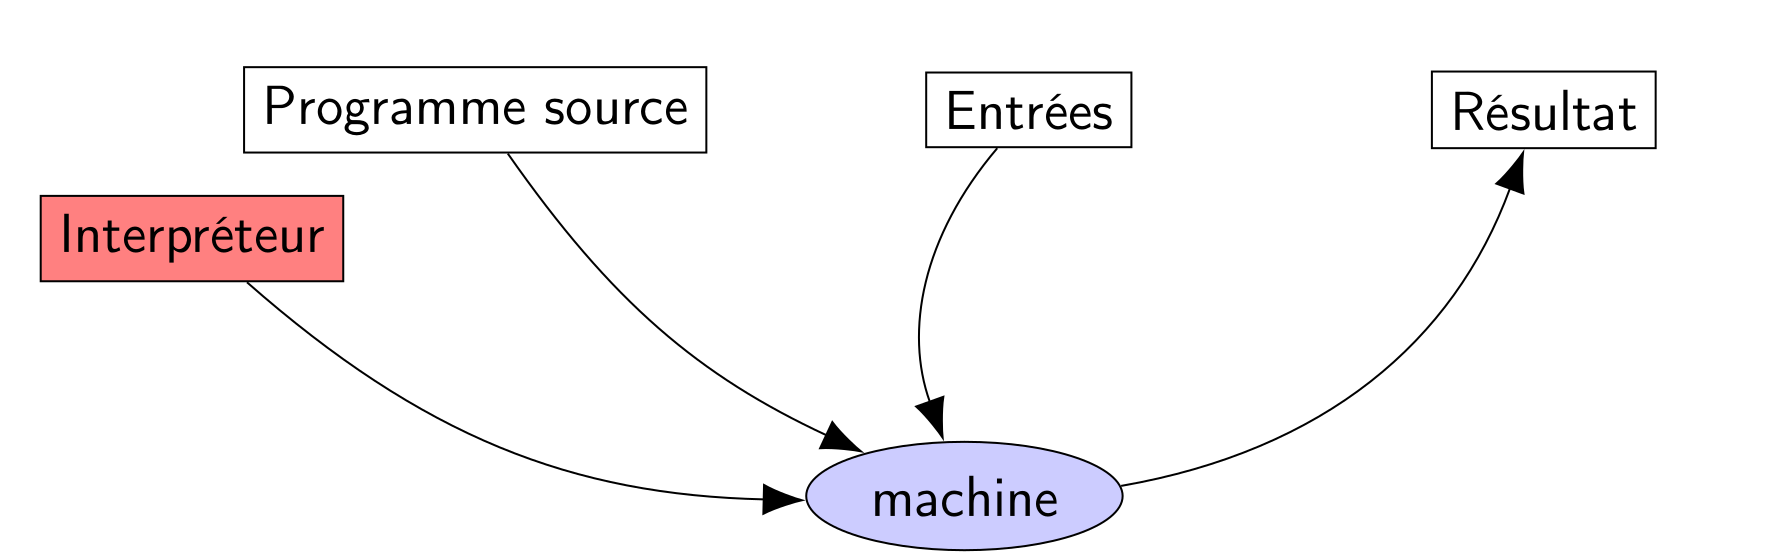
\includegraphics[scale=0.25]{ressources/interpreteur.png}

Source : \textit{Judicaël Courant}
\end{center}

\begin{minipage}{0.5\linewidth}
\begin{center}
\fbox{Mode interactif}

\begin{lstlisting}[style=compil]
>>> 1 + 2
3
>>> "1" + "2"
'12'
>>> "1" + 2
Traceback (most recent call last):
  File "<stdin>", line 1, in <module>
TypeError: can only concatenate str (not "int") to str

\end{lstlisting}

\end{center}
\end{minipage}\hfill
\begin{minipage}{0.5\linewidth}
\begin{center}
\fbox{Exécution d'un script Python}

\begin{lstlisting}[style=compil]
user@pc~$ python hello_world.py 
Hello world
\end{lstlisting}
\end{center}
\end{minipage}

\end{definition}

\begin{programme}{}

Voici un exemple de programme Python qui récupère des données sur son \textbf{entrée standard} (ici une saisie de l'utilisateur avec la fonction \texttt{input} mais ce pourrait être un fichier externe) , les traite puis renvoie des valeurs  sur sa \textbf{sortie standard} (ici la console utilisateur avec la fonction \texttt{print} mais ce pourrait être un fichier externe)   :


\begin{lstlisting}[style=rond]
#Définition de fonctions
def f(x):
    return x ** 2 - 3

## Programme principal

#entrées
a = float(input('Borne inférieure ? '))
b = float(input('Borne supérieure ? '))
s = float(input("Seuil de l'encadrement ?"))

#traitement 
while b - a > s: #boucle non bornée
    m = (a+b)/2  #affectation
    if f(m) < 0: #conditionnelle, branchement
        a = m
    else:
        b = m

#sorties
print(a, "<= racine(3) <= ", b)
\end{lstlisting}

\end{programme}


\begin{definition}{}

Un programme Python est un texte structuré comme une séquence d'\textbf{instructions}. 

Un interpréteur Python  exécute  le  programme sur un ordinateur en  mobilisant  des ressources de calcul (processeur) et de mémoire. 

L'exécution d'une instruction peut modifier \textbf{l'état courant du programme}, par \textbf{effet de bord}.   

Après l'exécution d'une instruction, l'interpréteur évalue par défaut l'instruction sur la ligne suivante (les lignes vides ne sont pas prises en compte) mais certaines instructions se traduisent par des sauts en avant (branchement) ou en arrière (boucle) dans le texte du programme.

Les séquences de caractères précédées d'un dièse \verb+#+ ne sont pas interprétées, ce sont des \textbf{commentaires}.



\end{definition}

\subsection{Environnements pour programmer en  Python}

\begin{manuel}{Environnement de programmation}
Lire les pages 3 à 5.
\end{manuel}

\begin{methode}{}

Pour programmer en Python, on peut :

\begin{itemize}[label=\ding{43}]

	\item Installer une distribution Python comprenant un interpréteur et un environnement de programmation : 
	\begin{itemize}
		\item la plus simple est Idle disponible sur le site officiel \href{https://docs.python.org/3/tutorial/datastructures.html}{Python} ;
				\item une distribution complète avec une interface simple et un débogueur très visuel : \url{https://thonny.org/} ;
		\item une distribution plus  lourde mais plus complète avec tous les modules scientifiques est \href{https://www.anaconda.com/products/individual}{Anaconda}.
\end{itemize}

\item Utiliser un interpréteur intégré au navigateur Web :

	\begin{itemize}
		\item \url{http://pythontutor.com/visualize.html#mode=edit} est idéal pour visualiser l'exécution du code mais propose peu de modules/bibliothèques externes ;
		\item \url{https://console.basthon.fr/} est plus riche en modules/bibliothèques externes.
			\item les activités \textbf{Capytale} partagées par les professeurs dans l'ENT (Ressources numériques) sont un autre moyen d'exécuter du code Python dans le navigateur.
\end{itemize}
\end{itemize}

\end{methode}


\subsection{Littéraux et types de base}


\begin{manuel}{Types de base}
\begin{itemize}[label=\ding{43}]
 \item Définitions  : page 30
 \item Exercice 1 : p. 42, QCM 4 p. 39
\end{itemize}
\end{manuel}


\begin{definition}{}
Un \textbf{littéral} est un texte qui est interprété par Python pour créer un \textbf{objet} en mémoire avec  une valeur bien spécifiée.

Un \textbf{objet} Python est caractérisé par son \textbf{identité}, son  \textbf{type} et sa \textbf{valeur}.

L'identifiant d'un objet s'obtient avec la fonction \texttt{id} et son type avec la fonction \texttt{type}.

\begin{lstlisting}[style=compil]
>>> id(842)
140200201318000
>>> type(842)
<class 'int'>
\end{lstlisting}

\end{definition}


\begin{methode}{}

Les objets de même type peuvent être combinés à l'aide d'opérateurs pour créer d'autres objets de même type. Certains opérateurs sont \textbf{polymorphes} et s'appliquent à des objets de types différents. Une opération entre des objets de types différents provoque  en général une erreur sauf pour des cas particuliers comme les types numériques pour lesquels il existe des règles de conversion implicite. Les quatre types de base sont :

\begin{tabular}{|c|c|c|c|}
\hline 
Type & Domaine de valeurs & Opérateurs & Exemple de littéraux \\ 
\hline 
\texttt{int} & entiers signés & \texttt{+  - * //   \%  **} & \texttt{0   -4   842} \\ 
\hline 
\texttt{float} & sous-ensemble des décimaux  & \texttt{+  - * /  **} & \texttt{0.0 -1.0 3.14} \\ 
\hline 
\texttt{bool} & valeurs logiques  & \texttt{not and or} & \texttt{True False} \\ 
\hline 
\texttt{str} & chaînes de caractères  & \texttt{+} & \texttt{'tb' ''  '2.4' 'Bonjour'} \\
\hline 
\end{tabular} 

On peut ajouter un type spécifique \texttt{None} sur lequel on ne définit pas d'opérateur car tous les objets de valeur \texttt{None} sont identiques.

\bcattention{} Dans le cas d'une combinaison de plusieurs opérateurs, des \textbf{règles de précédence} (ou priorité) déterminent l'ordre dans lequel les opérations sont effectuées. Les priorités usuelles des opérations algébriques sont bien connues (attention l'exponentiation a la plus haut priorité). On peut changer l'ordre de priorité en utilisant des \textbf{parenthèses}.  Pour les  opérations booléennes, les opérateurs classés par ordre décroissant de priorité sont  \texttt{not},  \texttt{and}  puis \texttt{or}.   

 

{\itshape Il est fortement recommandé d'utiliser des parenthèses qui sont l'opérateur de plus haute priorité, lorsqu'on n'est pas sûr des règle de précédence ou pour s'en affranchir. }



\end{methode}

\begin{exemple}{Opérations sur les types de base}

\begin{lstlisting}[style=compil]
>>> 11 + 3   #addition
14
>>> 11 * 3  #multiplication
33
>>> 11 ** 3 #exponentiation
1331
>>> 11 // 3  #quotient de la division euclidienne
3
>>> 11 % 3   #reste de la division euclidienne
2
>>> 11 / 3   #division décimale
3.6666666666666665
>>> not True  #négation booléenne
False
>>> True or False  #disjonction booléenne
True
>>> True and False  #conjonction booléenne
False
>>> '2' + 1    #impossible d'ajouter un 'str' et un 'int'
Traceback (most recent call last):
  File "<stdin>", line 1, in <module>
TypeError: can only concatenate str (not "int") to str
>>> '2' + '1'   #concaténation de 'str'
'21'
>>> not True and False    #not prioritaire sur and
False
>>> not(True and False)  #dans le doute on met des parenthèses
True
\end{lstlisting}

\end{exemple}


\subsection{Variable et expression}

\begin{definition}{}
Dans un programme pour manipuler des objets Python, on a besoin de les référencer par des noms.

Une \textbf{variable} est l'association entre un \textbf{nom} et un objet Python qu'on désigne souvent comme \textbf{valeur} de la variable.

L'opérateur \texttt{ = } réalise cette association. L'interpréteur Python évalue d'abord le membre de droite pour créer l'objet puis l'associe au membre de gauche contenant le \textbf{nom}. 


Cette \textbf{instruction} s'appelle une \textbf{affectation de variable}. Comme elle modifie \textbf{l'état courant} du programme on parle d'\textbf{effet de bord}.



\medskip

Voici les  représentations de  quelques  séquences d'affectations :


\begin{center}
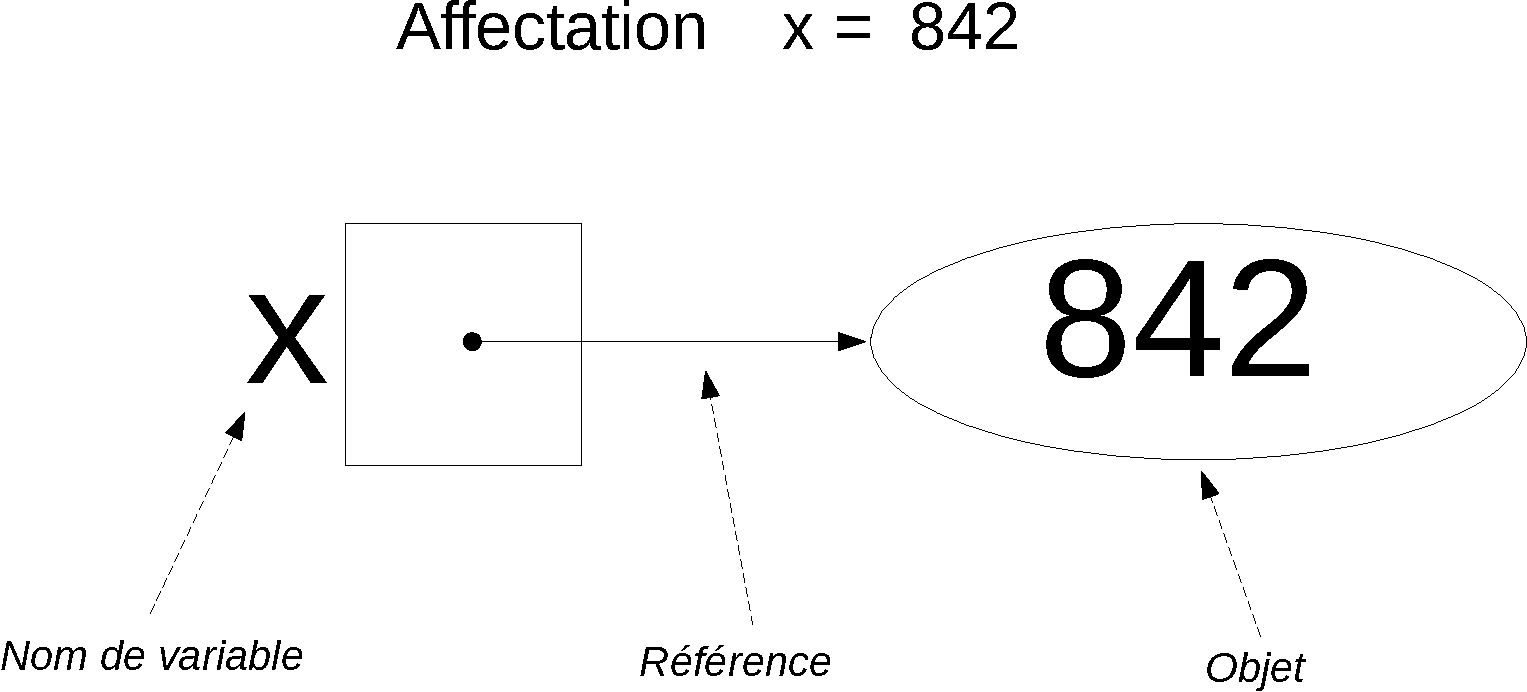
\includegraphics[scale=0.4]{ressources/affectation1-crop.pdf}
\end{center}

\hrule

\begin{center}
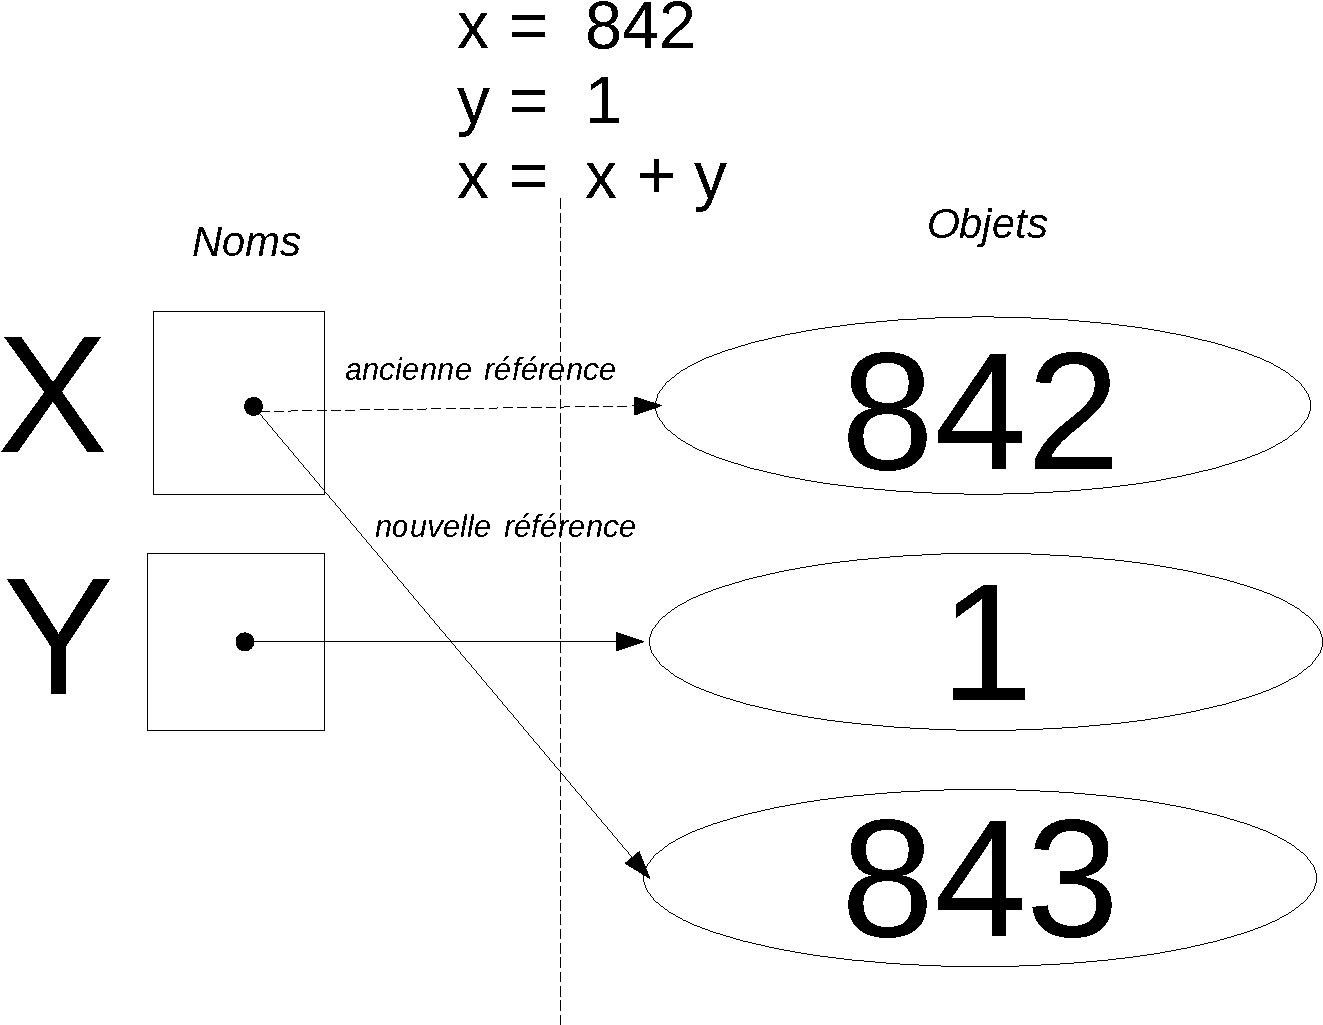
\includegraphics[scale=0.4]{ressources/affectation2-crop.pdf}
\end{center}


\hrule

\begin{center}
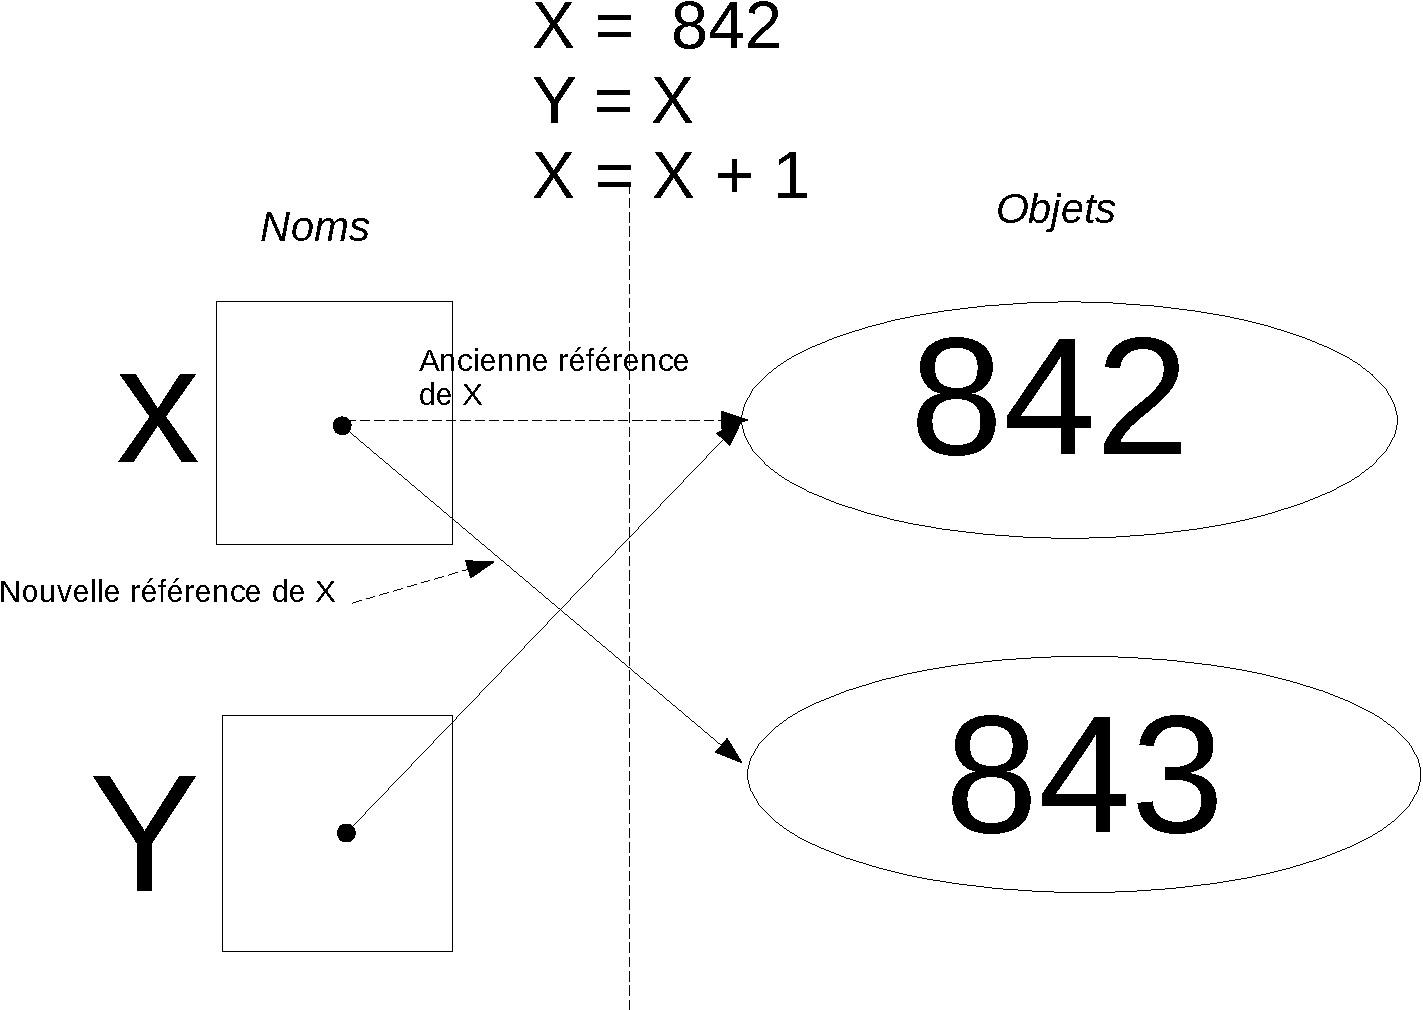
\includegraphics[scale=0.4]{ressources/affectation3-crop.pdf}
\end{center}


\end{definition}



\begin{definition}{}
Une \textbf{expression} est une combinaison de littéraux et de variables dont la valeur peut être évaluée par l'interpréteur en remplaçant les noms de variables par leur valeur.

Par exemple si dans l'état courant du  programme la valeur de \texttt{x} est 842 alors l'expression  \texttt{x + 1} a pour valeur 843.



\end{definition}


\begin{remarque}{}

\begin{itemize}
\item Les noms de variables en Python doivent obéir à certaines règles syntaxiques (ne pas commencer par un chiffre, ne peut pas contenir de tiret haut). Il est recommandé de les choisir en minuscules et d'utiliser le tiret bas comme séparateur si un nom est constitué de plusieurs mots comme \verb+compteur_vie+.

Pour plus de détails sur la syntaxe on pourra consulter la documentation \url{https://docs.python.org/3.9/reference/lexical_analysis.html} et pour les conventions de style la PEP 8 \url{https://www.python.org/dev/peps/pep-0008}.


\item L'instruction \texttt{x = x + 1} permet d'incrémenter la valeur de la variable \texttt{x} (à  condition qu'elle soit définie sinon cela provoque une erreur). 

\bcdanger{}  Dans une affectation, l'opérateur \texttt{ = } n'est pas un opérateur d'égalité et \texttt{x = x + 1} ne doit pas être interprété comme une égalité. Le \texttt{x} à  droite de l'opérateur représente la valeur associée précédemment au nom \texttt{x} tandis que le \texttt{x} à gauche est un nom auquel sera associée la valeur de l'expression \texttt{x + 1}. 

\end{itemize}

\end{remarque}

\begin{manuel}{Variables et expressions}
\begin{itemize}[label=\ding{43}]
 \item Définitions  : pages 30 et 31
 \item Exercices 3 et 4 p. 42, QCM questions 5 et 8  p. 39
\end{itemize}
\end{manuel}



\begin{methode}{}

Pour bien comprendre un programme on peut compléter un \textbf{tableau d'état} : on exécute le programme (en fixant éventuellement une instance d'entrée) comme le ferait l'interpréteur, en notant les valeurs de toutes les variables pour chaque instruction qui  une modifie  l'état de la mémoire par effet de bord.

Cet exemple classique permet de comprendre qu'il faut une variable de stockage pour sauvegarder la valeur de \texttt{a} si on veut échanger les valeurs des variables \texttt{a} et \texttt{b}

\begin{minipage}{0.4\linewidth}
\begin{lstlisting}[style=rond, numbers = left]
a = 842
b = 843
a = b
b = a
\end{lstlisting}
\end{minipage}\hfill
\begin{minipage}{0.55\linewidth}
\begin{tabular}{|c|c|c|}
\hline 
Instruction (numéro de ligne) & a & b \\ 
\hline 
ligne 1 & 842 &  \\ 
\hline 
ligne 2 & 842 & 843 \\ 
\hline 
ligne 3 & 843 & 843 \\ 
\hline 
ligne 4 & 843 & 843 \\ 
\hline 
\end{tabular} 
\end{minipage}

Pour échanger les valeurs des variables \texttt{a} et \texttt{b} on peut utiliser l'un des deux programme ci-dessous, celui de droite  plus pythonique utilise le déballage de \texttt{tuple}.


\medskip

\begin{minipage}{0.4\linewidth}
\begin{lstlisting}[style=rond, numbers = left]
a = 842
b = 843
c = a
a = b
b = c
\end{lstlisting}
\end{minipage}\hfill
\begin{minipage}{0.4\linewidth}
\begin{lstlisting}[style=rond, numbers = left]
a = 842
b = 843
a, b = b, a
\end{lstlisting}
\end{minipage}

\end{methode}


\begin{methode}{}

Étant donné deux variables de même type (celui de l'objet référencé), on peut :

\begin{itemize}
	\item répondre à la question \og{} \textit{Ont-elles la même valeur ?} \fg{} en les comparant  avec l'opérateur \texttt{ == }
	\item répondre à la question \og{} \textit{Référencent-elles le même objet ?} \fg{} en les comparant  avec l'opérateur \texttt{ is }
\end{itemize}

Deux variables peuvent avoir la même valeur sans référencer le même objet.

Si \texttt{a} est définie, l'instruction \texttt{c = a}  copie en \texttt{c}  la référence de \texttt{a}. Ainsi les noms \texttt{a} et \texttt{c} partagent une référence vers le même objet. 

En Python, la copie de variable se fait par \textit{aliasing} ou \textit{copie de référence}.

\begin{lstlisting}[style=compil]
>>> a = 842
>>> b = 843
>>> a == b
False
>>> a = a + 1
>>> a == b
True
>>> a is b
False
>>> c = a 
>>> a == a
True
>>> c is a
True
\end{lstlisting}

\end{methode}




\section{Instructions conditionnelles  (ou de branchement)}

\begin{manuel}{Conditionnelle}
\begin{itemize}[label=\ding{43}]
 \item Définition  : page 33
 \item Exercice 5 p. 42, QCM question 6  p. 39
\end{itemize}
\end{manuel}


\begin{exemple}{}

Le programme ci-dessous prend en entrée le crédit et le débit d'un compte bancaire, calcule le solde puis une pénalité de 10 \% du solde s'il est négatif. Le bloc du  \texttt{if} n'est exécuté que si le solde est négatif mais  le message \texttt{"Affichage de votre solde :"} s'affiche dans tous les cas.

\begin{lstlisting}[style=rond]
recette = float(input('Recette ?'))
debit = float(input('Débit ?'))
solde = recette - debit
if solde < 0:
	agios = solde * 0.1
	solde = solde + agio
print("Affichage de votre solde :")
\end{lstlisting}

On peut le compléter en affichant un message différent selon le signe du solde, le bloc du \texttt{else} s'exécute si et  seulement si la condition du \texttt{if} n'est pas vérifiée.

\begin{lstlisting}[style=rond]
if solde < 0:
	print("Solde débiteur : ", solde, "dont agios : ", agios)
else:
	print("Solde créditeur : ", solde)
\end{lstlisting}


Souvent on a besoin de considérer plus de deux alternatives, comme dans le programme ci-dessous qui affiche le tarif d'une entrée au musée en fonction de l'âge  :  gratuit pour les moins de 6 ans, sinon 5 euros pour les moins de 13 ans et sinon 8 euros.

\begin{lstlisting}[style=rond]
age = int(input('age ?'))
if age < 6:
	tarif = 0
elif age < 13:
	tarif = 5
else:
	tarif = 10
\end{lstlisting}


\end{exemple}


\begin{definition}{}

Dans l'exemple d'une résolution d'équation du second degré, des instructions de test permettent de choisir entre plusieurs branches pour continuer l'exécution du programme selon le signe du discriminant. La syntaxe générale des instructions de branchement est :

 
\begin{lstlisting}[style=rond]
if condition1:
    instruction       #
      ...             # bloc d'instructions 1
    instruction       #
elif condition2:
    instruction       #
      ...             # bloc d'instructions 2
    instruction       #
    instruction
elif ...
    .....
else :     
    instruction       #
      ...             # dernier bloc d'instructions 
    instruction       #

\end{lstlisting}

Seul le premier mot clé \verb+if+ est obligatoire, les autres \verb+elif+ et \verb+else+ sont optionnels. Noter que \verb+else+ n'est pas suivi d'une condition.

Les conditions sont des variables de type booléen ou des expressions qui sont évaluées sous forme de booléen. Attention, dans cette situation, Python évalue en booléen des types qui n'en sont pas a priori.

Si \verb+condition1+ a pour valeur \verb+True+ alors le bloc d'instructions 1 est exécuté. 

Si ce n'est pas le cas, \verb+condition2+ est évaluée. Si sa valeur est \verb+True+ alors le bloc d'instructions 2 est exécuté.

Sinon on passe au \verb+elif+ suivant et ainsi de suite.

Si aucune des conditions présentes derrière un des mot-clé \verb+elif+ n'est évaluée à \verb+True+alors le dernier bloc est exécuté. 

\textit{Remarque : Un seul des blocs d'instructions peut être exécuté : le premier possible ceci même si l'état courant rend plusieurs des conditions valides (\texttt{True}).}

Les conditions sont souvent construites à l'aide des opérateurs de comparaison et des opérateurs logiques  pour créer des expressions booléennes.

\begin{center}
\begin{tabular}{lcl}
\hline
\multicolumn{3}{c}{\textbf{Principaux opérateurs de comparaison de variables}} \\
& & \\
\texttt{x == y} &  & \texttt{x est égal à y} \\
\texttt{x != y} &  & \texttt{x est différent de y} \\
\texttt{x > y} &  & \texttt{x est strictement supérieur à y} \\
\texttt{x < y} &  & \texttt{x est strictement inférieur à y} \\
\texttt{x >= y} & & \texttt{x est  supérieur ou égal à y} \\
\texttt{x <= y} &  & \texttt{x est  inférieur ou égal à y} \\
\hline
\end{tabular}

\begin{tabular}{lcl}
\hline
\multicolumn{3}{c}{\textbf{Principaux opérateurs  sur des expressions booleenes}} \\
& & \\
\texttt{E and F} & & \texttt{Vraie si E est Vraie ET F est Vraie}\\
\texttt{E or F} & & \texttt{Vraie si E est Vraie OU F est Vraie }\\
\texttt{not E} &  & \texttt{Vraie si E est Fausse}\\
\hline
\end{tabular}
\end{center} 

{\itshape
\bcattention{} On peut combiner des opérateurs arithmétiques,  de comparaison  et logiques pour créer des expressions booléennes complexes. Il faut prêter attention aux \textbf{règles de précédence}. Les parenthèses sont prioritaires sur tous les autres opérateurs donc on peut les utiliser quand on n'est pas certain  des  \textbf{règles de précédence} ou pour s'en affranchir.

\begin{lstlisting}[style=compil]
>>> 3<4 and 5 == 2*2+1  #on fait confiance aux règles de précédence
True
>>> (3<4) and (5 == 2*2+1) #avec des  parenthèses, + sur et + lisible
True
\end{lstlisting}
}
\end{definition}


\begin{remarque}{}

Des tests de validation de données sont souvent utilisés. Dans l'exemple du tarif de cinéma, on peut souhaiter interrompre le  programme si l'âge saisi est  en dehors de la plage attendue ($[0;120]$ par exemple). On peut utiliser alors une instruction  \texttt{assert} selon la syntaxe   : \texttt{assert condition, "message"} qui reste silencieuse si la condition est vérifiée mais interrompt le programme sinon.

\begin{lstlisting}[style=compil]
>>> age = -10
>>> assert (age >= 0 and age <= 120), "valeur invalide"
Traceback (most recent call last):
  File "<stdin>", line 1, in <module>
AssertionError: valeur invalide
\end{lstlisting}

\texttt{assert condition, "message"} correspond à peu près à  :

\begin{lstlisting}[style=compil]
if not condition:
	exit("message")  #on sort du programme
#ici le programme continue
\end{lstlisting}

\end{remarque}

\section{Boucle bornée}


\begin{manuel}{Boucle bornée}
\begin{itemize}[label=\ding{43}]
 \item Définition  : page 34
 \item Exercices 7 et 8 p. 42, QCM question 10  p. 39
\end{itemize}
\end{manuel}


\begin{definition}{Boucle \texttt{for}}
Lorsque l'on veut répéter un certain nombre de fois un ensemble d'instructions on utilise la boucle inconditionnelle ou boucle \texttt{for} : 
 
\begin{minipage}{0.45\linewidth}
 \begin{programme}{}
 \begin{lstlisting}
 >>> for k in range(4):
		print("bonjour")
	
bonjour
bonjour
bonjour
bonjour
 \end{lstlisting}
 \end{programme}
 \end{minipage}
\hfill\begin{minipage}{0.45\linewidth}
 \begin{programme}{}
 \begin{lstlisting}
 >>> for k in range(4):
		print(k)
	
0
1
2
3
 \end{lstlisting}
 \end{programme}
 \end{minipage}

 Ici la fonction range renvoie un \emph{itérateur} qui produit consécutivement les valeurs entières de 0 à 3. La boucle \lstinline{for} ne fait que parcourir les valeurs de cet itérateur.  
 
 Plus généralement, la boucle \lstinline{for} permet de parcourir tout objet \emph{itérable} : 
 
\begin{minipage}{0.4\linewidth} %début texte
\begin{programme}{}
{\small
\begin{lstlisting}
>>> for c in 'AB':
		print(c)
	
A
B
\end{lstlisting}
}
\end{programme}
\end{minipage}
\hfill 
\begin{minipage}{0.6\linewidth} 
\begin{programme}{}
{\small
\begin{lstlisting}
>>> for x in [2, 6]:
		print(x**2)
	
4
36
\end{lstlisting}
}
\end{programme}
\end{minipage}

La syntaxe générale d'une boucle inconditionnelle \lstinline{for} est :

\begin{center}
\begin{minipage}{0.9\linewidth}
\begin{lstlisting}
for element in iterable:
    instruction    #
    instruction    # bloc d'instructions
    instruction    #
\end{lstlisting}
\end{minipage}
\end{center}
 
 La fonction \lstinline{range} possède trois arguments dont deux sont optionnels :
 
 \begin{itemize}
\item \texttt{range(n)} retourne un itérateur parcourant les entiers consécutifs entre 0 et \texttt{n} exclu.
\item \texttt{range(m,n)} retourne un itérateur parcourant les entiers consécutifs entre \texttt{m} compris  et \texttt{n} exclu.
\item \texttt{range(m,n,s)} retourne un itérateur parcourant les entiers consécutifs entre \texttt{m} compris  et \texttt{n} exclu avec un pas  de \texttt{s}.
\end{itemize}

\end{definition}


\begin{remarque}{}

En Python, le \textbf{bloc} d'une boucle inconditionnelle est délimité par :


\begin{itemize}
	\item Un \textbf{marqueur de début de bloc}, le caractère   \texttt{ : } à la fin de l'instruction définissant la boucle ;
	\item Une \textbf{indentation}  (décalage en espaces par rapport à la marge de gauche) commune à toutes les lignes d'instruction appartenant au bloc de la boucle.
\end{itemize}

Les instructions exécutées après la boucle ont un niveau d'indentation inférieur à celui du \textbf{bloc} de boucle.

\medskip

{\itshape 
En Python, \textbf{l'indentation} n'est pas un simple élément de présentation mais bien un élément de syntaxe, \texttt{IndentationError} est un message d'erreur classique   : }

\begin{lstlisting}[style=compil]
(base) fjunier@fjunier:~$ cat test.py
s  = 0
for k in range(10):
s = s + k
(base) fjunier@fjunier:~$ python3 test.py
  File "test.py", line 3
    s = s + k
    ^
IndentationError: expected an indented block
\end{lstlisting}

\end{remarque}

\begin{methode}{}

Le bloc d'une boucle  peut contenir une autre boucle, on parle alors de \textbf{boucles imbriquées}.


\begin{itemize}

\item Pour énumérer tous les couples $(i, j)$ avec $1 \leqslant i \leqslant 3$ et $1 \leqslant j \leqslant 3$, on peut écrire le programme \texttt{couple\_avec\_repetition.py} :

\begin{minipage}{0.45\linewidth}
\begin{lstlisting}[style=rond]
for i in range(1, 4):
    for j in range(1, 4):
        print(i, j)
\end{lstlisting}
\end{minipage}\hfill
\begin{minipage}{0.6\linewidth}
\begin{lstlisting}[style=compil]
1 1
1 2
1 3
2 1
2 2
2 3
3 1
3 2
3 3
\end{lstlisting}
\end{minipage}

\item Pour énumérer tous les couples $(i, j)$ avec $1 \leqslant i < j \leqslant 3$ , on peut écrire le programme \\ \texttt{couple\_ordre\_croissant.py} :

\begin{minipage}{0.48\linewidth}
\begin{center}
\begin{lstlisting}[style=rond]
for i in range(1,4):
    for j in range(i+1,4):
        print(i, j)
\end{lstlisting}
\end{center}
\end{minipage}\hfill
\begin{minipage}{0.5\linewidth}
\begin{center}
\begin{lstlisting}[style=compil]
fjunier@fjunier:~$ python3 couple_ordre_croissant.py 
1 2
1 3
2 3
\end{lstlisting}
\end{center}
\end{minipage}
\end{itemize}

\end{methode}

\section{Boucle non bornée}


\begin{manuel}{Boucle non bornée}
\begin{itemize}[label=\ding{43}]
 \item Définition  : page 34
 \item Exercices 6 et 9 p. 42, QCM question 6  p. 39
\end{itemize}
\end{manuel}

\begin{definition}{}


Dans une boucle \lstinline{for}, le nombre d'itérations est connue à l'avance (au plus tard lors de la première exécution de l'instruction). Lorsque l'on ne sait pas à l'avance combien de fois la boucle devra être exécutée, on utilise une boucle \lstinline{while}.

La syntaxe est la suivante : 


\begin{lstlisting}[style=rond]
while condition:
    instruction    #
    instruction    #   bloc d'instructions
    instruction    #
\end{lstlisting}

La \lstinline{condition} est une expression qui doit pouvoir être évaluée sous forme de booléen. Tant que sa valeur est True, le bloc d'instructions est exécuté.

\bcattention{} Lors de l'utilisation de \lstinline{while}, il faudra s'assurer que la condition finisse par prendre la valeur \texttt{False} sans quoi la boucle ne se terminera pas !!

\textit{Remarque : pour faire une opération jusqu'à la vérification d'une certaine condition il suffit d'ajouter l'opérateur logique \lstinline{not()}. }


\end{definition}



\begin{exemple}{}

\begin{itemize}

\item Un exemple classique est celui du calcul du PGCD de deux entiers \texttt{a} et \texttt{b} non tous nuls par la méthode d'Euclide.

\begin{lstlisting}[style=rond]
a = int(input('Entier a ?'))
b = int(input('Entier b ?'))
while b != 0:
	tmp = a
	a = b 
	b = tmp % b    #reste de la division euclidienne
print("PGCD : ", a)
\end{lstlisting}

\item Les algorithmes de seuil, sont un classique de l'enseignement de l'algorithmique dans le secondaire. Par exemple si on considère qu'une population augmente de 2 \% par an on peut déterminer le nombre d'années au bout duquel sa valeur initiale sera doublée avec le programme suivant : 

\medskip

\begin{lstlisting}[style=rond]
population = int(input("Population initiale ? "))
double = 2 * population
n = 0
taux = 2 / 100
while population < double:
	population = population * (1 + taux)
	n = n + 1
print("Doublement en ", n, "années")	
\end{lstlisting}

\end{itemize}
\end{exemple}

\vspace*{-15pt}

\begin{methode}{}

\begin{itemize}

\item On peut écrire volontairement une  \textbf{boucle infinie}, par exemple pour afficher un chronomètre :

\begin{lstlisting}[style=rond]
import time

compteur = 1
while True:		
	print(compteur)
	compteur = compteur + 1
	time.sleep(1)
\end{lstlisting}

\item On peut exécuter involontairement une \textbf{boucle infinie}, par exemple si on passe comme  paramètre un entier négatif à la fonction \verb+compte_a_rebours+ :


\begin{lstlisting}[style=rond]
import time

compteur = start
while compteur >= 0:
	print(compteur)		
	compteur = compteur - 1
	time.sleep(1)
\end{lstlisting}

\end{itemize}
\end{methode}




\section{Fonctions}

\subsection{Définir une fonction}


\begin{manuel}{Fonction}
\begin{itemize}[label=\ding{43}]
 \item Définition  : page 35
 \item Exercice 10 et 11 p. 42, QCM question 11  p. 39
\end{itemize}
\end{manuel}
 
 
\begin{definition}{}
Lorsqu'on a besoin de réutiliser tout un bloc  d'instructions, on peut l'encapsuler dans une \textbf{fonction}. On étend ainsi le langage avec une nouvelle instruction. Une fonction sert à factoriser et clarifier  le code, elle facilite la  maintenance et le partage. C'est un outil de \textbf{modularité}. 

Pour déclarer une fonction, on définit son \textbf{en-tête} (ou \textbf{signature}) avec  son \textbf{nom} et des \textbf{paramètres formels} d'entrée. Vient ensuite le bloc d'instructions,  décalé d'une indentation et qui constitue le \textbf{corps} de la fonction.

\begin{center}
\textbf{Fonction avec \texttt{return}}

\begin{lstlisting}[style=rond]
def mafonction(parametre1, parametre2): #signature
    bloc d'instructions (optionnel)
    return valeur
\end{lstlisting}


\textbf{Fonction sans \texttt{return}}

\begin{lstlisting}[style=rond]
def mafonction(parametre1, parametre2): #signature
    bloc d'instructions (non vide)
\end{lstlisting}
\end{center}


Si le corps de la  fonction contient au moins une instruction préfixée par le mot clef \texttt{return} alors l'exécution d'un \texttt{return}  termine l'exécution du corps de la fonction et renvoie une valeur au programme principal. Si le \texttt{return} est dans une structure de contrôle (boucle, test), il est possible que le corps de la fonction ne soit pas entièrement exécuté, on parle de \textbf{sortie prématurée}.

Une fonction sans \texttt{return} s'appelle une \textbf{procédure}, elle modifie l'état du programme principal par \textbf{effet de bord}. En Python, une procédure  renvoie quand même la valeur spéciale \texttt{None} au programme principal.  


\medskip

On exécute une fonction en substituant aux \textbf{paramètres formels} des valeurs particulières appelées \textbf{paramètres effectifs}.
On parle d'\textbf{appel de fonction}, on peut l'utiliser comme une \textbf{expression} si une valeur est renvoyée ou comme une \textbf{instruction} s'il s'agit d'une procédure. 


\end{definition}


 

Par exemple une fonction \texttt{carre} qui prend en paramètre un nombre \texttt{x} et qui renvoie son carré, s'écrira :

\begin{programme}{}
\begin{lstlisting}[style=rond]
def carre(x):
    return x ** 2
\end{lstlisting}
\end{programme}

Une fonction peut prendre plusieurs paramètres. Par exemple une fonction \verb+carre_distance_origine(x,y)+ qui prend en paramètres deux nombres \texttt{x} et \texttt{y} et qui renvoie le carré de la distance d'un point de coordonnées \texttt{(x, y)} à l'origine d'un repère orthonormal, s'écrira : 

\begin{programme}{}
\begin{lstlisting}[style=rond]
def carre_distance_origine(x, y):
    return x ** 2 + y ** 2
\end{lstlisting}
\end{programme}

Une fonction peut retourner un tuple de valeurs. Par exemple une fonction \verb+coord_vecteur+ qui prend en paramètres quatre nombres \texttt{xA, yA, xB, yB} et qui retourne les coordonnées du vecteur lié dont les extrémités ont pour coordonnées \texttt{(xA, yA)} et \texttt{(xB, yB)}, s'écrira : 

\begin{programme}{}
\begin{lstlisting}[style=rond]
def coord_vecteur(xA, yA, xB, yB):
    return (xB - xA, yB - yA)
\end{lstlisting}
\end{programme}


Voici un exemple de fonction sans paramètres d'entrée, ni  valeur de retour (il s'agit donc d'une procédure). 

\begin{programme}{}
\begin{lstlisting}[style=rond]
def message_defaite():
    print("Vous avez perdu, merci d'avoir participé") 
\end{lstlisting}
\end{programme}

\bcdanger{} Attention, \lstinline+return valeur+ renvoie \texttt{valeur} qu'on peut capturer dans une variable alors que \lstinline+print(valeur)+ affiche \texttt{valeur} sur la sortie standard (l'écran par défaut) mais \texttt{valeur} ne peut alors être capturée dans une variable. On donne ci-dessous un extrait de console Python, où on a défini maladroitement une fonction cube avec un \lstinline+print+ à la place d'un \lstinline+return+. On ne récupère pas la valeur de retour souhaitée mais \lstinline+None+ lorsqu'on appelle la fonction. 

\begin{lstlisting}[style=compil]
In [10]: def cube(x):
    ...:     print(x ** 3)
    ...:     

In [11]: cube(4)
64

In [12]: b = cube(5)
125

In [13]: b

In [14]: print(type(b))
<class 'NoneType'>

In [15]: print(b + 1)

TypeError: unsupported operand type(s) for +: 'NoneType' and 'int'
\end{lstlisting}

\subsection{Utiliser des bibliothèques de fonctions}

\begin{methode}{}
On a parfois besoin d'utiliser des fonctions de Python qui ne sont pas chargées pas défaut. Ces fonctions sont stockées dans des programmes Python appelées \textbf{modules} ou \textbf{bibliothèques}. Par exemple le module \texttt{math} contient les fonctions mathématiques usuelles et le module \texttt{random} contient plusieurs types de générateurs de nombres pseudo-aléatoires.

Pour importer une fonction d'un module on peut procéder de deux façons :
\begin{lstlisting}[language=python,title=Première façon]
#import du module de mathématique (création d'un point d'accès)
import math

#pour utiliser la fonction sqrt, on la préfixe du nom du module et d'un point
racine = math.sqrt(2)
\end{lstlisting}

\begin{lstlisting}[language=python,title=Deuxième façon]
#import de la fonction sqrt du module math
from math import sqrt

racine = sqrt(2)

#Pour importer toutes les fonctions de math, ecrire
#from math import *  
\end{lstlisting}

Pour obtenir de l'aide sur le module math dans la console Python, il faut d'abord l'importer avec \texttt{import math} puis taper \texttt{help(math)}, mais le mieux est encore de consulter la documentation en ligne \url{https://docs.python.org/3/}. Sans connexion internet, on peut   lancer en local  le serveur web de documentation avec la commande \texttt{python3 -m pydoc -b}.
 \end{methode}
 

 \begin{methode}{}
 
 
 
\begin{itemize}


\item Le module \texttt{random} rassemble diverses fonctions simulant le hasard :

\begin{center}
\begin{tabular}{|l|l|}
\hline 
Fonction & Spécification \\ 
\hline 
\texttt{random.randrange(a,b)} & renvoie un entier aléatoire dans [a;b[ \\ 
\hline 
\texttt{random.randint(a,b)} & renvoie un entier aléatoire dans [a;b] \\ 
\hline 
\texttt{random.random()} & renvoie un décimal aléatoire dans [0;1[ \\ 
\hline 
\texttt{random.uniform(a,b)} & renvoie un décimal aléatoire dans [a;b] \\ 
\hline 
\end{tabular} 


\end{center}


\item Le module \texttt{turtle} est une implémentation en \texttt{Python} du langage \texttt{Logo} créé dans les années 1970 pour l'enseignement de l'informatique à l'école. Il est disponible  dans la distribution standard de \texttt{Python}. 

En déplaçant une pointe de stylo qui peut être matérialisée par une tortue, on peut tracer des figures géométriques dans un repère cartésien dont l'origine est au centre de la fenêtre et dont l'unité par défaut est le pixel.  Lorsqu'on déplace le crayon, il laisse une trace s'il est baissé ou pas de trace s'il est levé.
	
Nous utiliserons les fonctions suivantes de \texttt{turtle}.

\begin{center}
	\begin{tabular}{|l|l|}
	\hline 
	Fonction & Spécification \\ 
	\hline 
	\texttt{turtle.goto(x,y)} & déplace la tortue jusqu'au point de coordonnées (x, y) \\
	\hline
	\texttt{turtle.penup()} & lever le crayon \\
	\hline
	\texttt{turtle.pendown()} & baisser le crayon \\
	\hline
	\texttt{turtle.setheading(angle)} & choisir l'angle d'orientation  de la tortue en degrés \\
	\hline 
	\texttt{turtle.forward(n)} & avancer de \texttt{n} pixels selon l'orientation de la tortue   \\
	\hline
	\texttt{turtle.left(a)} & tourne à gauche de \texttt{a} degrés   \\
	\hline
	\texttt{turtle.right(a)} & tourne à droite de \texttt{a}  degrés   \\
	\hline 
	\texttt{turtle.color("red")} & choisir la couleur rouge (ou "black", "green", "blue" \ldots)  \\
	\hline 
	\end{tabular} 
\end{center}

\end{itemize}

\end{methode}





\begin{exemple}{}
On donne ci-dessous un exemple d'utilisation du module \texttt{turtle}. On utilise un \texttt{import} avec renommage du module.

\begin{minipage}{0.65\linewidth}

\begin{programme}{}
\begin{lstlisting}[style=rond]
import turtle as tt

def spirale(n):
    tt.penup()
    tt.goto(0,0)
    tt.pendown()
    c = 5
    for i in range(4):
        for j in range(4):
            tt.forward(c)
            c = 10 + c
            tt.left(90)

spirale(4)
tt.exitonclick()
\end{lstlisting}
\end{programme}
\end{minipage}
\hfill
\begin{minipage}{0.3\linewidth}
\begin{center}
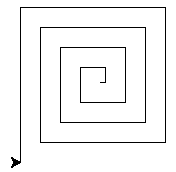
\includegraphics[scale=0.6]{ressources/boucle1.png}
\end{center}
\end{minipage}
\end{exemple}

%\newpage

\section{Erreurs}

\begin{manuel}{Erreurs}
\begin{itemize}[label=\ding{43}]
 \item Définitions page 37
 \item Exercice 13 p. 42.
\end{itemize}

\end{manuel}


\begin{definition}{}

On distingue plusieurs types d'\textbf{erreurs} ou \textbf{bugs} lors de l'exécution d'un programme Python. Le \textbf{débogage} d'un programme s'appuie d'abord sur la lecture attentive des messages d'erreurs de l'interpréteur et sur un traçage des valeurs par exemple en insérant des \texttt{print} ou en utilisant les outils de l'environnement de programmation (points d'arrêt, débogueur).

Python caractérise chaque erreur par un\textbf{ type}, voici les plus courants :
\begin{itemize}

	\item une \textbf{erreur de syntaxe} se produit lorsque la syntaxe du langage Python n'est pas respectée :
	
	\begin{lstlisting}[style=compil]
>>> 4 = a
  File "<stdin>", line 1
SyntaxError: cannot assign to literal
	\end{lstlisting}
	
	\item une \textbf{erreur de définition} se produit lorsqu'on évalue une expression avec des valeurs de variables non définies :

	\begin{lstlisting}[style=compil]
>>> 3 * a +1
Traceback (most recent call last):
  File "<stdin>", line 1, in <module>
NameError: name 'a' is not defined
	\end{lstlisting}
	
	\item une   \textbf{erreur de type} se produit lorsqu'on évalue une expression avec des valeurs de variables non définies :
	
	
	
	\begin{lstlisting}[style=compil]
>>> 2 + '2'
Traceback (most recent call last):
  File "<stdin>", line 1, in <module>
TypeError: unsupported operand type(s) for +: 'int' and 'str'
	\end{lstlisting}
	
	\item une \textbf{erreur d'exécution} se produit lorsque l'interpréteur ne peut pas évaluer une expression ou exécuter une instruction :
	
		\begin{lstlisting}[style=compil]
>>> def division(a, b):
...     return a / b
... 
>>> x = 8
>>> y = 0
>>> z = division(x, y)
Traceback (most recent call last):
  File "<stdin>", line 1, in <module>
  File "<stdin>", line 2, in division
ZeroDivisionError: division by zero
TypeError: unsupported operand type(s) for +: 'int' and 'str'
	\end{lstlisting}
	
	
\item une \textbf{erreur de logique} se produit lorsque le programme ne produit pas le résultat attendu ou ne se termine pas (boucle infinie) :


		\begin{lstlisting}[style=compil]
>>> x = 1
>>> while x > 0:
...     x = x +1      #boucle infinie, pour en sortir CTRL + C
^CTraceback (most recent call last):
  File "<stdin>", line 2, in <module>
KeyboardInterrupt

	\end{lstlisting}
	
\end{itemize}



\end{definition}


\begin{center}
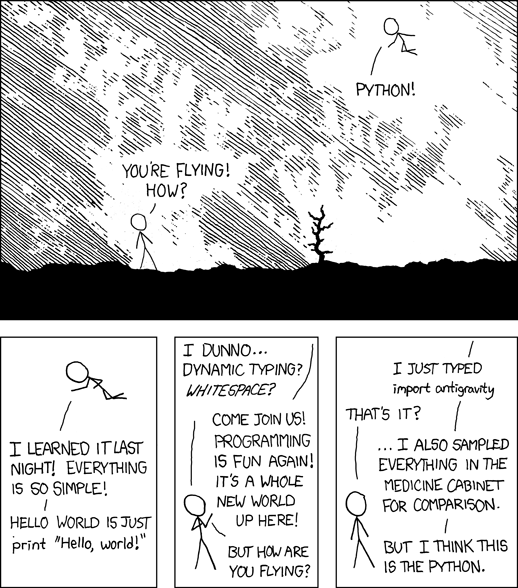
\includegraphics[scale=0.55]{ressources/python.png}

\href{https://www.explainxkcd.com/wiki/index.php/353:_Python}{XKCD : 353}
\end{center}

\newpage

\tableofcontents

 \end{document}
